% \documentclass{Thesis}
% \usepackage{fontspec}
% \setmainfont{Times New Roman}
% % XeLaTeX ашиглах учраас inputenc хэрэггүй
% %\usepackage[utf8]{inputenc}  

\documentclass[12pt, a4paper]{report}
\usepackage{graphicx}
\usepackage{multirow}
\usepackage[left=3cm, right=1.5cm, top=2cm, bottom=2cm]{geometry}
\setlength{\headheight}{14.92621pt}
\usepackage{fontspec}
\usepackage{titlesec}
\usepackage{setspace}
\usepackage{lipsum}
\usepackage{indentfirst}
\usepackage{array}
\usepackage{caption}
\usepackage{fancyhdr}
\usepackage{amssymb}
\newfontfamily\emojifont{Segoe UI Emoji}

\setmainfont{Times New Roman}[
  BoldFont = Times New Roman Bold,
  ItalicFont = Times New Roman Italic,
  BoldItalicFont = Times New Roman Bold Italic
]

\graphicspath{{Pictures}}

\newcommand{\nmct}{{Шинэ Монгол Технологийн Коллеж}}
\newcommand{\universityname}{{ШИНЭ МОНГОЛ ТЕХНОЛОГИЙН КОЛЛЕЖ}}
\newcommand{\departmentname}{{КОМПЬЮТЕРИЙН УХААНЫ ТЭНХИМ}}
\newcommand{\titlename}{{13-р зууны Монголын түүхийг таниулах систем}} 
\newcommand{\authorsname}{{Наранбаатар БАТТҮВШИН}}
\newcommand{\authorShort}{{Н.Баттүвшин}}
\newcommand{\studentID}{{s21c061b}}
\newcommand{\supervisorname}{{Б.Батчулуун}}
\newcommand{\cityname}{{Улаанбаатар хот}}
\newcommand{\gradYear}{{\the\year{} он}}

\renewcommand{\contentsname}{Гарчиг}
\renewcommand{\chaptername}{Бүлэг}
\renewcommand{\listtablename}{Хүснэгтийн жагсаалт}
\renewcommand{\listfigurename}{Зургийн жагсаалт}
\renewcommand{\tablename}{Хүснэгт}
\renewcommand{\figurename}{Зураг}

% Зураг болон хүснэгтийн дугаарлалтыг 1-ээс эхлүүлэх
\renewcommand{\thefigure}{ \arabic{figure}}
\renewcommand{\thetable}{\arabic{table}}

% Хүснэгтийн caption-ийг доор байрлуулах
\captionsetup[table]{position=bottom, skip=5pt}
\captionsetup[figure]{position=bottom, skip=5pt}

\titleformat{\chapter}[hang]
	{\bfseries\huge}
	{\chaptername~\thechapter.}
	{1em}
	{}

% Хуудасны толгой тохиргоо - бүлгийн нэрийг харуулах
\pagestyle{fancy}
\fancyhf{}
\fancyhead[R]{\leftmark}
\fancyfoot[C]{\thepage}
\renewcommand{\headrulewidth}{0.4pt}
\renewcommand{\chaptermark}[1]{\markboth{\chaptername~\thechapter.~#1}{}}

% Бүлгийн эхний хуудсанд ч толгой харуулах
\fancypagestyle{plain}{
  \fancyhf{}
  \fancyhead[R]{\leftmark}
  \fancyfoot[C]{\thepage}
  \renewcommand{\headrulewidth}{0.4pt}
}

\begin{document}
	
	\thispagestyle{empty}
\onehalfspacing

% Title page
\hspace{-15mm}
\begin{minipage}[h]{0.2\textwidth}
	
\includegraphics[width=\textwidth]{NMCT.png}
\end{minipage}
\hfill
\begin{minipage}[h]{0.7\textwidth}
	\centering
	\large
	\MakeUppercase{\textbf{
		 \nmct \\
		 \departmentname
	}}
\end{minipage}

\par
	\begin{tabular}{@{\hspace{85mm}}r l}
		Оюутаны код: & \studentID \\
		Оюутан овог нэр: & \authorsname \\
	\end{tabular}

\begin{center}
	\vspace*{50mm}
	{\doublespacing\MakeUppercase{
		\textbf{\Large \titlename} \\
		 \textbf{/Дэд бакалаврын төгсөлтийн судалгааны ажил}
	}}
	\par
	\vspace{5mm}
	\begin{tabular}{l @{\hspace{75mm}} l}
		Удирдсан багш: & \supervisorname, Магистр \\
		Гүйцэтгэсэн оюутан: & \studentID, \authorShort \\
	\end{tabular}
	\vspace*{\fill}
\end{center}
\begin{center}
	\cityname \\
	\gradYear
\end{center}

\newpage
\thispagestyle{empty}

\begin{minipage}{\textwidth}
	\raggedright
	\hspace{15mm}
	\large
	\MakeUppercase{\textbf{
		\nmct \\
		\hspace{25mm}
		\departmentname
	}}
\end{minipage}

\par

\begin{center}
	\vspace*{65mm}
	
	{\doublespacing\MakeUppercase{
		\textbf{Төгсөлтийн судалгааны ажил} \\
		\textbf{\Large \titlename} \\
	}}
	\par
	\vspace{35mm}
	\begin{tabular}{l l}
		\textbf{Гүйцэтгэгч:}\authorShort \\
		\textbf{Удирдагч:} \supervisorname, Магистр\\
		
	\end{tabular}
	\vspace*{\fill}
\end{center}
\begin{center}
	\cityname \\
	\gradYear
\end{center}
	\newpage
\setcounter{page}{1}
\thispagestyle{empty}   
\begin{center}
\begin{minipage}{\textwidth}
    \centering
    \large
    \MakeUppercase{\textbf{
     \vspace{1cm}
     \noindent\rule{\textwidth}{0.4pt} 
         \titlename \\} }
         \authorShort \\
        \departmentname \\
        \studentID@nmct.edu.mn
\end{minipage}
\thispagestyle{empty}

\noindent\textbf{Хураангуй:}
{\hspace{135mm}}    
\vspace{3mm}
\begin{flushleft}
\hspace{1em}13-р зууны Монголын эзэнт гүрний түүхийг (Чингис хаан, байлдан дагуулалт, соёл)
интерактив мобайл апп-аар таниулах төсөл нь залуу үеийнхэнд түүхийн мэдлэгийг түгээх, сонирхлыг нэмэгдүүлэхэд
чиглэсэн. Апп нь Flutter-ээр хөгжүүлэгдэж, оффлайн горимд (SQLite) ажиллах бөгөөд онлайн болоход Firebase-ээр sync 
хийнэ. Гол функцууд: түүхэн хүмүүсийн намтар, интерактив газрын зураг, цагийн хэлхээс, квиз, мультимедиа. Дизайн нь модульчлагдсан 
(UI, Data, Logic), аюулгүй (AES шифрлэлт, биометр баталгаажуулалт). Төсөл Agile аргачлалаар 8 сарын хугацаатай хэрэгжинэ. 
UML диаграммууд (Use Case, Sequence, System) болон SRS, SDD баримт бичгүүд бэлэн. Үр дүн: Монгол хэл дээрх боловсролын
дижитал нөөцийг баяжуулах, түүхийн мэдлэгийг хүртээмжтэй болгох.
\end{flushleft}

\vspace{3mm}

\noindent\textbf{Түлхүүр үгс:} 13-р зуун, Монголын түүх, Интерактив апп,Flutter хөгжүүлэл
\end{center}
	
	% Ром тоогоор дугаарлах хэсэг эхлэх
	\pagenumbering{roman}
	
	\newpage
	\singlespacing
	\tableofcontents
	\thispagestyle{fancy}												
	\newpage
\thispagestyle{empty}

\section*{Товчилсон үгсийн жагсаалт}
\addcontentsline{toc}{chapter}{Товчилсон үгсийн жагсаалт}

\begin{tabular}{@{}l p{12cm}}
\textbf{API} & Application Programming Interface \\
\textbf{APK} & Android Package Kit \\
\textbf{CI/CD} & Continuous Integration / Continuous Deployment \\
\textbf{CRUD} & Create, Read, Update, Delete \\
\textbf{ERD} & Entity Relationship Diagram \\
\textbf{FK} & Foreign Key \\
\textbf{GUI} & Graphical User Interface \\
\textbf{iOS} & iPhone Operating System \\
\textbf{JSON} & JavaScript Object Notation \\
\textbf{KPI} & Key Performance Indicator \\
\textbf{MVC} & Model-View-Controller \\
\textbf{NoSQL} & Not Only SQL \\
\textbf{PK} & Primary Key \\
\textbf{SDK} & Software Development Kit \\
\textbf{SDLC} & Software Development Life Cycle \\
\textbf{SQL} & Structured Query Language \\
\textbf{SQLite} & SQL Lite (Lightweight Database) \\
\textbf{SRS} & Software Requirements Specification \\
\textbf{UI} & User Interface \\
\textbf{UML} & Unified Modeling Language \\
\textbf{URL} & Uniform Resource Locator \\
\textbf{UX} & User Experience \\
\end{tabular}

	\newpage
	\singlespacing
	\listoffigures
	\thispagestyle{fancy}
	\newpage
	\listoftables
	\thispagestyle{fancy}
	\setlength{\headheight}{14.92621pt}
\newpage
\thispagestyle{empty}

\section*{Ажлын төлөвлөгөө}
\addcontentsline{toc}{chapter}{Ажлын төлөвлөгөө}

\begin{table}[h]
\centering
\small
\begin{tabular}{|p{0.8cm}|p{5.5cm}|p{2cm}|p{2cm}|p{3cm}|p{1cm}|}
\hline
\textbf{д/д} & \textbf{Гүйцэтгэх ажлын нэр} & \textbf{Эхлэх хугацаа} & \textbf{Дуусах хугацаа} & \textbf{Гайбор} & \textbf{Явц} \\
\hline
1 & Сэдэв сонгох, удирдагч багштай зөвлөлдөх, судалгааны үндэслэл боловсруулах & 2025.09.01 & 2025.09.24 & Сэдэв, удирдагч багш, зорилго, зорилт тодорхойлох & 100\% \\
\hline
2 & Түүхийн эх сурвалж цуглуулах, судалгааны тойм, онолын үндэслэл бичих & 2025.09.24 & 2025.10.24 & Монголын нууц товчоо, Britannica, онолын үндэслэл & 100\% \\
\hline
3 & Судалгааны төлөвлөгөө, апп-ын шаардлага, дизайн (UI/UX, ERD) боловсруулах & 2025.10.24 & 2025.12.05 & Төлөвлөгөө, SRS, UI/UX, ERD & 100\% \\
\hline
4 & Өгөгдлийн сангийн дизайн хийх, SQLite төлөвлөх & 2025.11.25& 2025.12.01& SQLite өгөгдлийн сан & 100\% \\
\hline
5 & ТСА Үзлэг 1 & 2025.12.02 & 2025.12.04 & Үзлэг 1 &  \\
\hline
6 & Програмчлалын орчин бэлтгэх, үндсэн функцууд кодлох & 2026.01.02 & 2026.02.06 & Хөгжүүлэлтийн орчин, үндсэн функцууд & \\
\hline
7 & Интерактив элемент, цагийн хэлхээс хөгжүүлэх & 2026.02.06 & 2026.02.27 & Цагийн хэлхээс &  \\
\hline
8 & Газрын зургийн модуль, Quiz ба тоглоомын модуль кодлох & 2026.02.27 & 2026.03.27 & Газрын зураг, Quiz, тоглоом &  \\
\hline
9 & Мультимедиа цуглуулга нэмэх & 2026.03.27 & 2026.04.10 & Зураг, видео, аудио & \\
\hline
10 & Апп-ын туршилт, оффлайн дэмжлэг, аюулгүй байдал хэрэгжүүлэх & 2026.04.10 & 2026.04.24 & Unit тест, оффлайн, шифрлэлт & \\
\hline
11 & Хэрэглэгчийн интерфейс сайжруулах, бета туршилт & 2026.04.24 & 2026.05.08 & UI сайжруулалт, бета туршилт & \\
\hline
12 & ТСА Үзлэг 2: Апп-ын демо үзүүлэх, санал авах & 2026.03.01& 2026.03.03& Үзлэг 2 &  \\
\hline
13 & Туршилтын үр дүнг дүн шинжилгээ хийх, апп-ын алдаа засах & 2026.05.08 & 2026.05.15 & Дүн шинжилгээ, алдаа засалт &  \\
\hline
14 & Баримт бичиг шинэчлэх, гарын авлага боловсруулах, урьдчилсан хамгаалалт & 2026.04.12 & 2026.04.21  & Баримт бичиг, урьдчилсан хамгаалалт & \\
\hline
15 & Эцсийн тайлан боловсруулах, ТСА үндсэн хамгаалалт & 2026.05.22 & 2026.05.29& Эцсийн тайлан, үндсэн хамгаалалт & \\
\hline
\end{tabular}
\end{table}

\vspace{1cm}

\begin{minipage}[t]{0.45\textwidth}
\raggedright
Удирдагч багш: \\
Гүйцэтгэсэн оюутан:
\end{minipage}
\hfill
\begin{minipage}[t]{0.45\textwidth}
\raggedleft
/\supervisorname, Магистр/ \\
/\studentID/ \authorShort/
\end{minipage}

	
	% Араб тоогоор дугаарлах хэсэг эхлэх (Удиртгал-аас)
	\newpage
	\pagenumbering{arabic}
	
	\newpage
	
	\pagestyle{plain}
	\setcounter{page}{1}
	
	\chapter{Удиртгал}
	\section{Үндэслэл, ач холбогдол}
	
	Өнөө үед дижитал технологи залуу үеийн өдөр тутмын амьдралын салшгүй хэсэг болж, мэдлэг мэдээллээ олж авах үндсэн сувгуудын нэг болсон. Ухаалаг гар утас, таблет болон онлайнаар дамжих контентууд уламжлалт сурах бичиг, хэвлэмэл номоос хамаагүй түгээмэл хэрэглэгддэг болжээ. Ялангуяа өсвөр үе болон оюутан залуучуудын хувьд мэдээлэл авах хэлбэр цахим хэрэглээ рүү шилжсэн ч, тэдэнд зориулсан чанартай, системтэй, интерактив боловсролын аппликэйшн Монгол хэл дээр хангалттай түгээмэл бус байна.

Монголын түүх нь дэлхийн түүхэнд онцгой байр суурь эзэлдэг хэр нь залуучуудад ойлгомжтой, сонирхол татахуйц, дижитал хэлбэрээр хүрэх боломж хомс хэвээр байна. Одоогоор Монгол хэл дээрх боловсролын апп-ууд цөөн, контентын чанар болон интерактив байдал сул, хэрэглэгчдийг удаан хугацаанд татах боломж хязгаарлагдмал байдаг. Үүнээс шалтгаалж залуус түүхийн мэдлэгээ гүнзгийрүүлэхээс илүү богино хэмжээний, түр зуурын анхаарал татсан контентууд руу ханддаг болсон.

Тиймээс энэхүү төсөл нь зөвхөн нэгэн апп бүтээх зорилготой бус, харин Монголын түүхийг орчин үеийн технологийн шийдлээр баяжуулж, залуу үедээ хүртээмжтэй, сонирхолтой хэлбэрээр хүргэхэд чиглэнэ. Интерактив визуал контент, тоглоомын элемэнт, түвшин ахих систем зэрэг нь хэрэглэгчдийн сурах сонирхлыг нэмэгдүүлж, түүхийн талаарх мэдлэг, үндэсний ухамсрыг бодитоор дэмжих боломжтой.

Ингэснээр уг систем нь боловсролын салбарт дижитал шинэчлэл хийх, Монголын түүхийг илүү өргөн хүрээнд түгээх, залуу үеийн түүхийн мэдлэгийг нэмэгдүүлэх зэрэг олон талын ач холбогдолтой гэж үзэж байна.
	
	\section{Зорилго, зорилт}
	
	\subsection*{Зорилго}
	
	13-р зууны Монголын түүхийг таниулах интерактив апп бүтээх замаар залуу үеийнхэнд түүхийн мэдлэгийг түгээх, сонирхлыг нэмэгдүүлэх. Энэ нь түүхийн боловсролыг дижитал хэлбэрээр хүртээмжтэй болгох, Монгол хэл дээрх боловсролын нөөцийн дутагдлыг нөхөхөд чиглэнэ.
	
	\newpage
	\subsection*{Зорилт}
	
	\begin{enumerate}
		\item Түүхийн эх сурвалж судлах, мэдээлэл цуглуулах.
		\item Апп-ын шаардлага, дизайныг тодорхойлох (SRS, UI/UX, ERD).
		\item Flutter ашиглан кросс-платформ апп бүтээх.
		\item SQLite-д өгөгдөл хадгалах, Firebase-ээр онлайн sync хийх.
		\item Туршилт явуулж, хэрэглэгчийн санал хүсэлтээр сайжруулах.
		\item Үр дүнг дүгнэж, цаашдын өргөтгөлийг төлөвлөх.
	\end{enumerate}

	\section{Системийн функцууд}
	
	Апп нь дараах үндсэн функцуудыг агуулна:
	
	\begin{table}[h]
	\centering
	\begin{tabular}{|p{1.5cm}|p{5cm}|p{7cm}|}
	\hline
	\textbf{Код} & \textbf{Функц} & \textbf{Тайлбар} \\
	\hline
	FR-01 & Түүхэн хүмүүсийн намтар & Чингис хаан, Өгэдэй зэрэг хүмүүсийн намтар, зураг харуулах \\
	\hline
	FR-02 & Байлдан дагуулалтын газрын зураг & Интерактив газрын зураг, зум хийх, тулаан дээр дарах \\
	\hline
	FR-03 & Цагийн хэлхээс & Үйл явдлуудыг цаг хугацаагаар харуулах timeline \\
	\hline
	FR-04 & Квиз & Мэдлэг шалгах асуулт хариулт, оноо цуглуулах \\
	\hline
	FR-05 & Мультимедиа & Зураг, видео, аудио үзэх \\
	\hline
	FR-06 & Гэр бүлийн мод & Хаадын гэр бүлийн мод харуулах \\
	\hline
	FR-07 & Соёлын мэдээлэл & Соёл, нийгмийн амьдралын мэдээлэл \\
	\hline
	\end{tabular}
	\caption{Системийн функцуудын жагсаалт}
	\label{tab:functions}
	\end{table}

	\section{Хэрэглэгчийн зорилтот бүлэг}
	
	\begin{itemize}
		\item \textbf{Үндсэн хэрэглэгч:} Залуучууд, сурагчид, оюутнууд (13+ насны)
		\item \textbf{Нэмэлт хэрэглэгч:} Багш нар, түүх судлаачид
	\end{itemize}
	
	Хэрэглэгчид нь Монгол хэл мэдэх, Android эсвэл iOS мобайл төхөөрөмжтэй байх шаардлагатай.

	\setlength{\headheight}{27pt}
\newpage
\pagestyle{plain}
\chapter{Судалгааны сэдвийн онол,\\ өнөөгийн түвшин}

\section{Судалгааны сэдвийн онол}

Судалгааны сэдэв нь боловсролын зорилготой мобайл апп хөгжүүлэлтэд чиглэсэн бөгөөд онолын үндэслэл нь дижитал боловсролын платформ бүтээхэд тулгуурладаг.

\subsection{Дижитал боловсролын онол (e-Learning Theory)}

Өнөөгийн дижитал эринд мобайл апп нь боловсролын мэдлэг түгээх гол хэрэгсэл болсон бөгөөд энэ нь дижитал боловсролын онолд суурилдаг. Энэ онол нь мэдлэгийг интерактив, хүртээмжтэй байдлаар хүргэхэд чиглэдэг бөгөөд constructivism (бүтээгдэхүйн онол)-ын зарчмаар хэрэглэгч өөрөө мэдлэг бүтээх боломж олгодог (жишээ: квиз, газрын зураг ашиглан судлах).

\subsection{Mobile Learning (m-Learning) онол}

Mobile learning онол нь мобайл төхөөрөмжийн давуу талыг (оффлайн ажиллах, интерактив элемент) ашиглаж, суралцагчийг хаана ч, хэзээ ч сурах боломжтой болгодог. Энэ онолын үүднээс апп нь:

\begin{itemize}
	\item \textbf{Gamification:} Тоглоомын элемент (оноо цуглуулах, шагнал) ашиглан хэрэглэгчийн анхаарлыг татах
	\item \textbf{Personalization:} Хувийн тохиргоо (түвшин сонгох) хийх
\end{itemize}

\subsection{Програм хангамжийн хөгжүүлэлтийн онол}

Онолын хүрээнд апп хөгжүүлэлт нь Software Development Life Cycle (SDLC)-ийн загварыг дагадаг:

\begin{enumerate}
	\item Шаардлага тодорхойлох (SRS)
	\item Дизайн (UI/UX, өгөгдлийн сан)
	\item Хөгжүүлэлт
	\item Туршилт
	\item Хамгаалалт
\end{enumerate}

Энэ нь Agile аргачлалаар хэрэгжинэ, учир нь боловсролын апп-д хэрэглэгчийн санал хүсэлтэд тулгуурлан байнга шинэчлэх шаардлагатай.

\subsection{Өгөгдлийн сангийн онол}

Өгөгдлийн сангийн онол нь relational database model (хүснэгтүүдийн хоорондын харилцаа: one-to-many, жишээ: Person → Event) ашиглаж, өгөгдлийг үр дүнтэй хадгалах, авахад чиглэдэг.

\subsection{Аюулгүй байдлын онол}

Аюулгүй байдлын онол нь CIA triad (Confidentiality, Integrity, Availability)-д суурилж, өгөгдлийг шифрлэх, баталгаажуулах арга хэмжээ авна.

\section{Өнөөгийн түвшин}

2025 оны байдлаар мобайл апп хөгжүүлэлт, ялангуяа боловсролын апп-ын түвшин өндөр хөгжсөн бөгөөд кросс-платформ технологи (Flutter, React Native) голлох байр суурь эзэлж байна.

\begin{table}[h]
\centering
\begin{tabular}{|p{4cm}|p{9cm}|}
\hline
\textbf{Чиг хандлага} & \textbf{Тайлбар} \\
\hline
Gamification & Retention-ийг 30-40\% нэмэгдүүлдэг (Duolingo, Khan Academy) \\
\hline
AI Personalization & Хувийн санал болгох, recommendation system \\
\hline
AR/VR элемент & Интерактив туршлага өгөх \\
\hline
Оффлайн дэмжлэг & Local DB + cloud sync ашиглах \\
\hline
Кросс-платформ & Апп-уудын 30\% Flutter/React Native ашигладаг \\
\hline
\end{tabular}
\caption{Боловсролын апп-ын өнөөгийн чиг хандлага}
\label{tab:trends}
\end{table}

Монгол Улсад мобайл апп хөгжүүлэлт өсөн нэмэгдэж байгаа ч боловсролын зорилготой апп-ууд (Ulger, Mongolian Script Apps) цөөн, ихэвчлэн статик контенттэй байгаа тул интерактив апп-ын дутагдал бий.

\section{Flutter Framework}

Flutter нь Google-ийн бүтээсэн кросс-платформ фреймворк бөгөөд нэг код ашиглан Android, iOS, вэб, desktop апп хөгжүүлэх боломж олгодог.

\begin{table}[h]
\centering
\begin{tabular}{|p{6cm}|p{7cm}|}
\hline
\textbf{Давуу тал} & \textbf{Сул тал} \\
\hline
Hot Reload - код өөрчилсөн үед UI шууд шинэчлэгдэх & Native функц (камер) шаардлагатай үед plugin шаардана \\
\hline
Widget-based UI - Card, ListView, TimelineTile & Апп-ын хэмжээ native-ээс арай том \\
\hline
Performance - native ARM код руу compile & Learning curve - Dart хэл сурах шаардлага \\
\hline
Хөгжүүлэлтийн цагийг 40-50\% багасгадаг & \\
\hline
\end{tabular}
\caption{Flutter-ийн давуу болон сул талууд}
\label{tab:flutter}
\end{table}

2025 оны байдлаар Flutter 3.38 хувилбартай, 1 сая+ хөгжүүлэгчтэй, кросс-платформ апп-уудын 30\%-ийг эзэлж байна.

\section{Firebase Platform}

Firebase нь Google-ийн cloud-based платформ бөгөөд апп-ын backend (сервергүй) шийдэл өгдөг.

\textbf{Гол функцууд:}
\begin{itemize}
	\item \textbf{Firestore/Realtime DB:} Түүхэн өгөгдлийг cloud-д хадгалах, sync хийх
	\item \textbf{Storage:} Зураг/видео/аудио хадгалах
	\item \textbf{Authentication:} Биометр + PIN баталгаажуулалт
	\item \textbf{Cloud Functions:} Sync conflict шийдэх
	\item \textbf{AI Logic:} ML Kit ашиглан текст таних, recommendation
\end{itemize}

\section{SQLite Database}

SQLite нь lightweight, embedded relational өгөгдлийн сан бөгөөд мобайл апп-д зориулагдсан, сервер шаардлагагүй.

\begin{table}[h]
\centering
\begin{tabular}{|p{4cm}|p{9cm}|}
\hline
\textbf{Онцлог} & \textbf{Тайлбар} \\
\hline
Zero-configuration & Суулгах тохиргоо шаардлагагүй \\
\hline
ACID compliant & Найдвартай транзакци баталгаажуулах \\
\hline
Small footprint & 500KB library \\
\hline
Өргөн хэрэглээ & 1 тэрбум+ төхөөрөмжид суусан \\
\hline
\end{tabular}
\caption{SQLite-ийн онцлог шинж чанарууд}
\label{tab:sqlite}
\end{table}

2025 оны байдлаар SQLite файл формат 2050 он хүртэл тогтвортой, Android-ийн албан ёсны guide дагуу ашиглагддаг.
	\newpage
\pagestyle{plain}
\chapter{Судалгааны арга зүй}

\section{SDLC ба Agile аргачлал}

Судалгааны арга зүй нь боловсролын зорилготой мобайл апп хөгжүүлэлтийн төслийн үндэс болох бөгөөд энэ нь програм хангамжийн хөгжүүлэлтийн амьдралын мөчлөгийн (SDLC - Software Development Life Cycle) загварыг дагаж, Agile аргачлалаар хэрэгжинэ.

Agile нь уян хатан, итератив (давталттай) хөгжүүлэлтэд чиглэдэг бөгөөд хэрэглэгчийн санал хүсэлтэд тулгуурлан байнга шинэчлэх боломж олгодог. Энэ арга зүй нь төслийг үе шатаар хувааж, эрсдлийг бууруулж, чанарыг баталгаажуулдаг.

\subsection{Судалгааны үе шатууд}

\begin{table}[htbp]
\centering
\begin{tabular}{|p{0.8cm}|p{4cm}|p{8cm}|}
\hline
\textbf{№} & \textbf{Үе шат} & \textbf{Тайлбар} \\
\hline
1 & Судалгаа ба шаардлага цуглуулах & SRS баримт бичиг боловсруулах, функционал болон функционал бус шаардлага жагсаах \\
\hline
2 & Дизайн & UML диаграммууд (use case, sequence, ERD) зурах, UI/UX дизайн (Figma) хийх \\
\hline
3 & Хөгжүүлэлт & Flutter ашиглан код бичих, SQLite-д өгөгдөл хадгалах, Firebase-ээр sync хийх \\
\hline
4 & Туршилт & Unit testing, integration testing, usability testing (10-20 хүн) \\
\hline
5 & Үнэлгээ ба шинэчлэлт & KPI хэмжих, A/B testing хийх \\
\hline
6 & Deployment & Google Play, App Store-д байршуулах, CI/CD ашиглах \\
\hline
\end{tabular}
\caption{Судалгааны арга зүйн үе шатууд}
\label{tab:sdlc}
\end{table}

\newpage
\section{Модулийн дизайн}

Аппыг модульчлагдсан архитектурт суурилан хөгжүүлэх бөгөөд энэ нь хөгжүүлэлтийг илүү үр ашигтай болгоно. Модулиудыг бие даасан байдлаар зохион байгуулж, хоорондын хамаарлыг багасгасан.

\begin{table}[htbp]
\centering
\begin{tabular}{|p{3cm}|p{4cm}|p{3cm}|p{3cm}|}
\hline
\textbf{Модуль} & \textbf{Үүрэг} & \textbf{Технологи} & \textbf{Хамаарал} \\
\hline
UI Module & Дэлгэц харуулах & Flutter Widgets & Business Logic \\
\hline
Data Module & Өгөгдөл хадгалах & SQLite & Network \\
\hline
Business Logic & Логик боловсруулах & Dart & UI, Data \\
\hline
Network Module & Онлайн sync & Firebase & Data \\
\hline
\end{tabular}
\caption{Модулийн тохиргоо}
\label{tab:modules}
\end{table}

\section{Өгөгдлийн сангийн дизайн}

Өгөгдлийн сан нь relational байх бөгөөд түүхэн өгөгдлийг хадгалахад зориулагдсан. SQLite ашиглах, entity relationships: One-to-many.

\begin{table}[htbp]
\centering
\begin{tabular}{|p{2cm}|p{7cm}|p{4cm}|}
\hline
\textbf{Хүснэгт} & \textbf{Багана} & \textbf{Тайлбар} \\
\hline
Persons & person\_id (PK), name, birth\_date, death\_date, description, image\_url & Түүхэн хүмүүсийн мэдээлэл \\
\hline
Events & event\_id (PK), title, date, description, person\_id (FK) & Үйл явдлууд \\
\hline
Maps & map\_id (PK), title, coordinates, event\_id (FK) & Газрын зургийн өгөгдөл \\
\hline
Quizzes & quiz\_id (PK), question, answers, correct\_answer & Квиз асуултууд \\
\hline
Media & media\_id (PK), type, url, related\_id (FK) & Мультимедиа файлууд \\
\hline
\end{tabular}
\caption{Өгөгдлийн сангийн хүснэгтийн бүтэц}
\label{tab:database}
\end{table}

\section{Системийн тохиргоо}

\subsection{Front-End}

Flutter framework ашиглан UI/UX дизайн хийх. Интерфейс нь Material Design эсвэл Cupertino загварыг дагаж, Монгол хэл дээр ажиллана. Оффлайн кэшинг ашиглан хурдан ажиллах.

\subsection{Back-End}

Firebase ашиглан өгөгдөл sync хийх. Голчлон оффлайн тул local logic дээр суурилсан, онлайн болоход шинэ контент татах.

\newpage
\subsection{Өгөгдлийн сан}

\begin{itemize}
	\item \textbf{Local:} SQLite
	\item \textbf{Cloud:} Firestore
\end{itemize}

\section{Хамгаалалтын дизайн}

Оффлайн апп-д зориулсан аюулгүй байдлын арга хэмжээ:

\begin{table}[htbp]
\centering
\begin{tabular}{|p{4cm}|p{9cm}|}
\hline
\textbf{Арга хэмжээ} & \textbf{Тайлбар} \\
\hline
AES-256 шифрлэлт & Локал өгөгдлийг шифрлэх \\
\hline
Биометр/PIN & Local authentication ашиглах \\
\hline
Input validation & SQL injection-ээс сэргийлэх \\
\hline
Keystore & API key-г аюулгүй хадгалах \\
\hline
Permissions & Зөвхөн шаардлагатай зөвшөөрөл авах \\
\hline
\end{tabular}
\caption{Хамгаалалтын арга хэмжээнүүд}
\label{tab:security}
\end{table}

\section{UML диаграммууд}

\subsection{Use Case Diagram}


Use case diagram нь апп-ын хэрэглэгчийн үйлдлийг (actor → use case) харуулдаг. Апп-д actor (User) болон use case-ууд (Газрын зураг үзэх, Квиз тоглох, Намтар унших) зурдаг.

\begin{figure}[htbp]
\centering
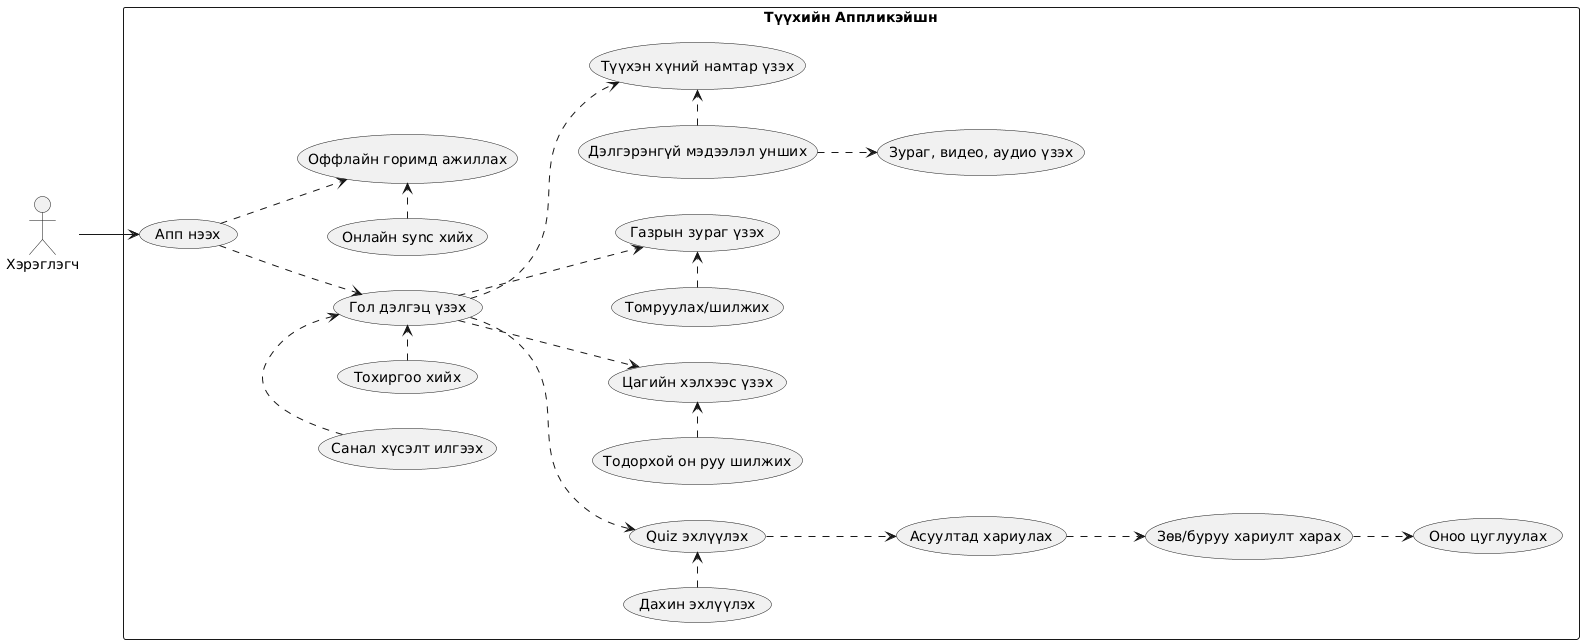
\includegraphics[width=\textwidth]{use_case.png}
\caption{Use Case диаграмм}
\label{fig:usecase}
\end{figure}
\newpage
\subsection{Sequence Diagram}

Sequence diagram нь UML-ийн хэсэг бөгөөд апп-ын объектуудын хоорондын харилцан үйлдлийг цаг хугацааны дарааллаар харуулдаг. Апп-д хэрэглэгч намтар үзэх үед (User → UI → Provider → DB → Firebase) ямар дарааллаар ажиллахыг тодорхойлдог.

\begin{figure}[htbp]
\centering
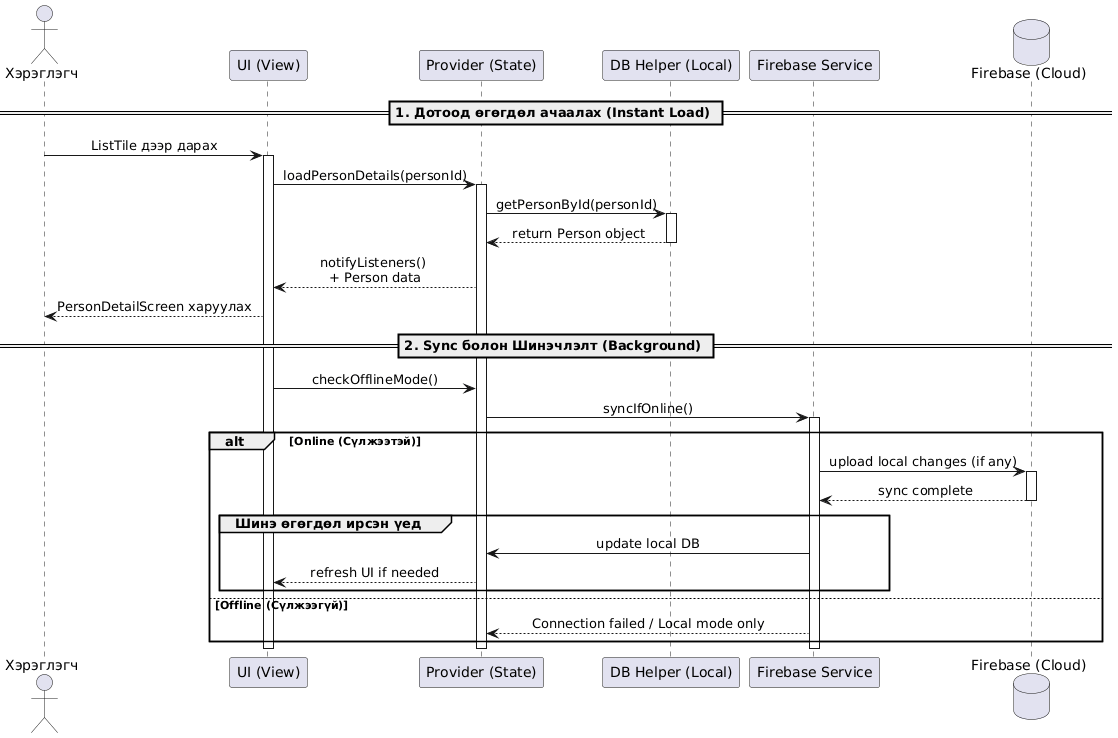
\includegraphics[width=\textwidth]{sequence_diagram.png}
\caption{Sequence диаграмм}
\label{fig:sequence}
\end{figure}
\subsection{System Diagram}

System diagram нь апп-ын ерөнхий архитектурыг (компонент, холбоос, өгөгдлийн урсгал) харуулдаг. Апп-д tier-үүдийг (Client: Flutter UI, Data: SQLite + Firebase) тодорхойлдог.

\begin{figure}[htbp]
\centering
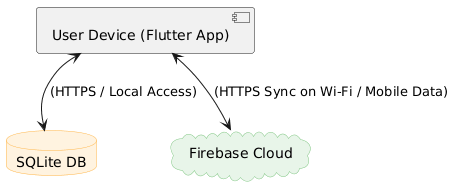
\includegraphics[width=0.7\textwidth]{system_diagram.png}
\caption{Системийн диаграмм}
\label{fig:system}
\end{figure}
\newpage
\subsection{ERD Diagram}

ERD (Entity-Relationship Diagram) нь өгөгдлийн сангийн бүтцийг (entity, attribute, relationship) харуулдаг. Persons (name, description) → Events (title, date) one-to-many холбоос зурдаг.

\begin{figure}[htbp]
\centering
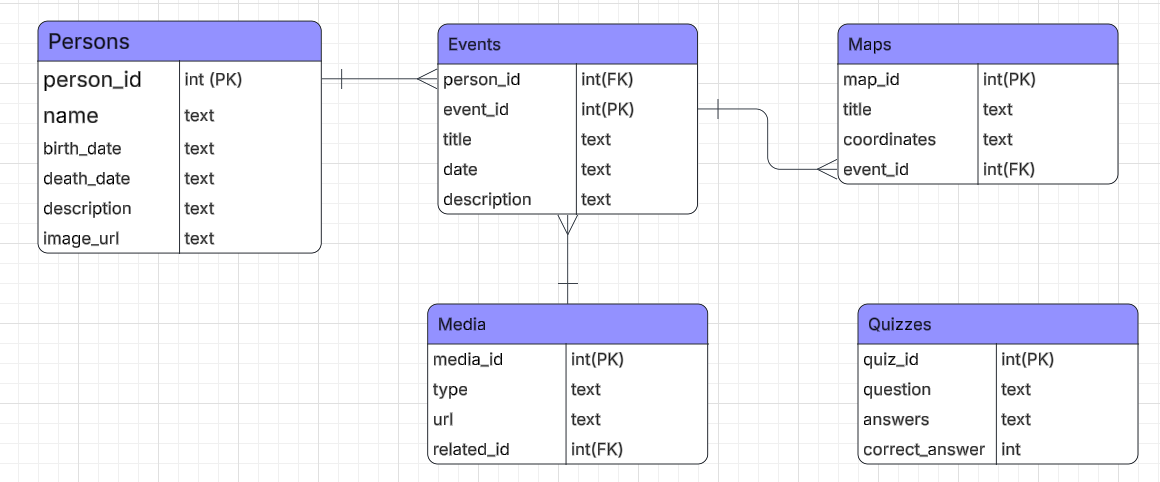
\includegraphics[width=\textwidth]{er_diagram.png}
\caption{ERD диаграмм}
\label{fig:erd}
\end{figure}
\section{Хэрэглэгдэх технологи}

\begin{table}[htbp]
\centering
\begin{tabular}{|p{3cm}|p{5cm}|p{5cm}|}
\hline
\textbf{Технологи} & \textbf{Хувилбар} & \textbf{Зориулалт} \\
\hline
Flutter & 3.38+ & Кросс-платформ UI хөгжүүлэлт \\
\hline
Dart & 3.0+ & Програмчлалын хэл \\
\hline
SQLite & 3.x & Локал өгөгдлийн сан \\
\hline
Firebase & Latest & Cloud sync, authentication \\
\hline
Figma & Latest & UI/UX дизайн \\
\hline
Git/GitHub & Latest & Version control, CI/CD \\
\hline
\end{tabular}
\caption{Хэрэглэгдэх технологийн жагсаалт}
\label{tab:tech}
\end{table}
	\newpage
\pagestyle{plain}
\chapter{Хэрэгжүүлэлт}

Энэхүү бүлэгт 13-р зууны Монголын түүхийг таниулах мобайл аппликейшний хөгжүүлэлтийн үйл явцыг дэлгэрэнгүй тайлбарлана. Аппын эх код нь Flutter фреймворкийн дагуу бүтэцлэгдсэн бөгөөд Dart програмчлалын хэл дээр бичигдсэн. Хэрэгжүүлэлтийг хөгжүүлэлтийн орчин, төслийн бүтэц, өгөгдлийн загварчлал (Model), үйлчилгээний давхарга (Service), төлөвийн удирдлага (State Management), дэлгэцүүд (Screen), дахин ашиглагдах компонент (Component), мөн Firebase интеграцийн гэсэн дэс дарааллаар авч үзнэ.

%% ============================================================
\section{Хөгжүүлэлтийн орчин ба хэрэгслүүд}
%% ============================================================

Аппыг хөгжүүлэхэд ашигласан үндсэн орчин, хэрэгслүүдийн мэдээллийг доорх хүснэгтэд харуулав.

\begin{table}[htbp]
\centering
\begin{tabular}{|p{3.5cm}|p{3.5cm}|p{6.5cm}|}
\hline
\textbf{Хэрэгсэл} & \textbf{Хувилбар} & \textbf{Зориулалт} \\
\hline
Flutter SDK & 3.38+ & Кросс-платформ UI фреймворк \\
\hline
Dart & 3.0+ & Програмчлалын хэл \\
\hline
Android Studio & Latest & Android эмулятор, APK бүтээх \\
\hline
VS Code & Latest & Код засварлагч (Editor) \\
\hline
Firebase & Latest & Cloud синхрончлол, баталгаажуулалт \\
\hline
Git / GitHub & Latest & Хувилбарын удирдлага (Version Control) \\
\hline
Figma & Latest & UI/UX дизайн зурах \\
\hline
\end{tabular}
\caption{Хөгжүүлэлтийн орчин ба хэрэгслүүд}
\label{tab:dev_tools}
\end{table}

Төслийн \texttt{pubspec.yaml} тохиргооны файлд зарласан гол хамаарлуудыг (dependencies) дараах хүснэгтэд жагсаав.

\begin{table}[htbp]
\centering
\begin{tabular}{|p{4cm}|p{2.5cm}|p{7cm}|}
\hline
\textbf{Сан (Package)} & \textbf{Хувилбар} & \textbf{Зориулалт} \\
\hline
\texttt{firebase\_core} & \texttt{\^{}2.24.2} & Firebase платформыг эхлүүлэх \\
\hline
\texttt{cloud\_firestore} & \texttt{\^{}4.14.0} & Cloud Firestore өгөгдлийн сан \\
\hline
\texttt{provider} & \texttt{\^{}6.1.1} & Төлөвийн удирдлага (State Management) \\
\hline
\texttt{google\_fonts} & \texttt{\^{}6.1.0} & Google шрифтүүдийг ашиглах \\
\hline
\texttt{flutter\_earth\_globe} & \texttt{\^{}2.2.0} & 3D бөмбөрцөг газрын зураг \\
\hline
\texttt{lucide\_flutter} & \texttt{\^{}0.563.0} & Нэмэлт дүрс тэмдэгт (Icons) \\
\hline
\end{tabular}
\caption{Төслийн гол хамаарлууд (dependencies)}
\label{tab:dependencies}
\end{table}

%% ============================================================
\section{Төслийн бүтэц}
%% ============================================================

Flutter төслийн эх код нь \texttt{lib/} хавтас дотор байрлах бөгөөд модульчлагдсан архитектурын дагуу зохион байгуулагдсан. Төслийн бүтцийг доорх хүснэгтэд харуулав.

\begin{table}[htbp]
\centering
\begin{tabular}{|p{4cm}|p{9.5cm}|}
\hline
\textbf{Хавтас / Файл} & \textbf{Тайлбар} \\
\hline
\texttt{lib/main.dart} & Аппын оролтын цэг (Entry Point), Firebase эхлүүлэлт, Provider тохиргоо \\
\hline
\texttt{lib/models/} & Өгөгдлийн загвар классууд (Person, Event, Quiz, MapData, Media, EmpireTerritory) \\
\hline
\texttt{lib/services/} & Үйлчилгээний давхарга (DataService, InsightService) \\
\hline
\texttt{lib/providers/} & Төлөвийн удирдлагын класс (AppProvider) \\
\hline
\texttt{lib/screens/} & Дэлгэцийн виджетүүд (7 дэлгэц) \\
\hline
\texttt{lib/components/} & Дахин ашиглагдах UI компонентууд (7 компонент) \\
\hline
\texttt{assets/data/} & JSON өгөгдлийн файлууд (persons, events, maps, quizzes, culture) \\
\hline
\texttt{assets/images/} & Зураг, дүрслэлийн файлууд \\
\hline
\texttt{assets/maps/} & Газрын зургийн текстур зургууд \\
\hline
\end{tabular}
\caption{Төслийн хавтасны бүтэц}
\label{tab:project_structure}
\end{table}

%% ============================================================
\section{Аппын оролтын цэг — main.dart}
%% ============================================================

\texttt{main.dart} файл нь аппын эхлэл цэг (entry point) бөгөөд дараах үндсэн үүргүүдийг гүйцэтгэдэг:

\begin{enumerate}
	\item \textbf{Firebase эхлүүлэлт:} \texttt{Firebase.initializeApp()} функцээр Firebase платформыг ачааллаж, cloud үйлчилгээнүүдтэй холбогдох бэлтгэл хангана.
	\item \textbf{Provider бүртгэл:} \texttt{MultiProvider} ашиглан \texttt{InsightService} болон \texttt{AppProvider} гэсэн хоёр \texttt{ChangeNotifier}-ийг бүртгэж, аппын аль ч хэсгээс хандах боломжтой болгоно.
	\item \textbf{MaterialApp тохиргоо:} Google Fonts (Inter) шрифт, цагаан суурь өнгө бүхий загварчлалыг тодорхойлж, \texttt{HomeScreen}-ийг нүүр дэлгэц болгон тохируулна.
\end{enumerate}

\texttt{HomeScreen} нь \texttt{StatefulWidget} бөгөөд \texttt{initState()} дотор \texttt{AppProvider.loadAllData()} функцийг дуудаж, бүх оффлайн өгөгдлийг програм эхлэхэд нэг удаа ачааллана. Нүүр дэлгэц нь \texttt{Stack} виджет ашиглан дараах бүрэлдэхүүн хэсгүүдийг давхарлан харуулна:

\begin{itemize}
	\item \texttt{HeaderCarousel} — Зурагт карусель (auto-scroll)
	\item \texttt{QuickActions} — Түргэн холбоос товчнууд
	\item \texttt{HistoryInsightCard} — AI-д суурилсан түүхийн мэдлэгийн карт
	\item \texttt{FeaturedContent} — Онцлох түүхүүдийн жагсаалт
	\item \texttt{TopActionBar} — Хайлт ба мэдэгдлийн товчнууд
	\item \texttt{BottomNav} — Доод навигацийн самбар
\end{itemize}

%% ============================================================
\section{Өгөгдлийн загварчлал (Models)}
%% ============================================================

Аппын өгөгдлийн давхарга нь 6 загвар класс (Model)-аас бүрдэнэ. Загвар бүр нь \texttt{fromMap()} factory constructor ашиглан JSON өгөгдлийг Dart объект болгон хөрвүүлэх, \texttt{toMap()} ашиглан буцаагаар хөрвүүлэх, мөн \texttt{copyWith()} ашиглан хуулбар үүсгэх чадвартай.

\subsection{Person загвар}

Түүхэн хүмүүсийн мэдээллийг хадгалах загвар класс.

\begin{table}[htbp]
\centering
\begin{tabular}{|p{3cm}|p{3cm}|p{7.5cm}|}
\hline
\textbf{Талбар} & \textbf{Төрөл} & \textbf{Тайлбар} \\
\hline
\texttt{personId} & \texttt{int?} & Хүний дугаар (Primary Key) \\
\hline
\texttt{name} & \texttt{String} & Нэр \\
\hline
\texttt{birthDate} & \texttt{String?} & Төрсөн огноо \\
\hline
\texttt{deathDate} & \texttt{String?} & Нас барсан огноо \\
\hline
\texttt{description} & \texttt{String} & Намтар, тайлбар \\
\hline
\texttt{imageUrl} & \texttt{String?} & Зургийн зам \\
\hline
\end{tabular}
\caption{Person загварын талбарууд}
\label{tab:person_model}
\end{table}

\subsection{Event загвар}

Түүхэн үйл явдлуудыг хадгалах загвар класс. \texttt{personId} талбар нь тухайн үйл явдалтай холбоотой хүнийг зааж өгнө (Foreign Key).

\begin{table}[htbp]
\centering
\begin{tabular}{|p{3cm}|p{3cm}|p{7.5cm}|}
\hline
\textbf{Талбар} & \textbf{Төрөл} & \textbf{Тайлбар} \\
\hline
\texttt{eventId} & \texttt{int?} & Үйл явдлын дугаар (PK) \\
\hline
\texttt{title} & \texttt{String} & Гарчиг \\
\hline
\texttt{date} & \texttt{String} & Огноо \\
\hline
\texttt{description} & \texttt{String} & Тайлбар \\
\hline
\texttt{personId} & \texttt{int?} & Холбоотой хүний дугаар (FK) \\
\hline
\end{tabular}
\caption{Event загварын талбарууд}
\label{tab:event_model}
\end{table}

\subsection{Quiz загвар}

Мэдлэг шалгах квиз асуултуудыг хадгалах загвар. Хариултууд нь JSON форматтай тэмдэгт мөр (String) хэлбэрээр хадгалагдана.

\begin{table}[htbp]
\centering
\begin{tabular}{|p{3.5cm}|p{2.5cm}|p{7.5cm}|}
\hline
\textbf{Талбар} & \textbf{Төрөл} & \textbf{Тайлбар} \\
\hline
\texttt{quizId} & \texttt{int?} & Квизийн дугаар (PK) \\
\hline
\texttt{question} & \texttt{String} & Асуултын текст \\
\hline
\texttt{answers} & \texttt{String} & Хариултуудын JSON массив \\
\hline
\texttt{correctAnswer} & \texttt{int} & Зөв хариултын индекс (0--3) \\
\hline
\end{tabular}
\caption{Quiz загварын талбарууд}
\label{tab:quiz_model}
\end{table}

\subsection{MapData загвар}

Газрын зургийн өгөгдлийг хадгалах загвар. Координат, он цаг, өнгө зэрэг мэдээллийг агуулна.

\begin{table}[htbp]
\centering
\begin{tabular}{|p{3cm}|p{3cm}|p{7.5cm}|}
\hline
\textbf{Талбар} & \textbf{Төрөл} & \textbf{Тайлбар} \\
\hline
\texttt{mapId} & \texttt{int?} & Газрын зургийн дугаар (PK) \\
\hline
\texttt{title} & \texttt{String} & Нэр \\
\hline
\texttt{coordinates} & \texttt{String} & Координат (өргөрөг, уртраг) \\
\hline
\texttt{eventId} & \texttt{int?} & Холбоотой үйл явдлын дугаар (FK) \\
\hline
\texttt{description} & \texttt{String?} & Тайлбар \\
\hline
\texttt{year} & \texttt{String?} & Он цаг \\
\hline
\texttt{color} & \texttt{String?} & Маркерийн өнгө \\
\hline
\end{tabular}
\caption{MapData загварын талбарууд}
\label{tab:mapdata_model}
\end{table}

\subsection{Media загвар}

Мультимедиа файлуудын (зураг, видео, аудио) мэдээллийг хадгалах загвар.

\begin{table}[htbp]
\centering
\begin{tabular}{|p{3cm}|p{3cm}|p{7.5cm}|}
\hline
\textbf{Талбар} & \textbf{Төрөл} & \textbf{Тайлбар} \\
\hline
\texttt{mediaId} & \texttt{int?} & Медиа дугаар (PK) \\
\hline
\texttt{type} & \texttt{String} & Төрөл: image, video, audio \\
\hline
\texttt{url} & \texttt{String} & Файлын зам (URL) \\
\hline
\texttt{relatedId} & \texttt{int?} & Холбоотой объектийн дугаар (FK) \\
\hline
\end{tabular}
\caption{Media загварын талбарууд}
\label{tab:media_model}
\end{table}

\subsection{EmpireTerritory загвар}

Монголын эзэнт гүрний нутаг дэвсгэрийн хил хязгаар болон байлдан дагуулалтын цэгүүдийг статик өгөгдөл хэлбэрээр хадгалах класс. Энэ нь 3D бөмбөрцөг болон 2D газрын зургийн аль алинд ашиглагддаг.

\texttt{EmpireTerritory} класс нь хоёр үндсэн статик өгөгдөл агуулна:

\begin{itemize}
	\item \texttt{boundaryCoords} — Эзэнт гүрний хил хязгаарын полигон координат (өргөрөг, уртраг хосууд). Зүүн Европоос Зүүн Азийн эргийг хүртэлх 36 координатын цэгээс бүрдэнэ.
	\item \texttt{markers} — Түүхэн байлдан дагуулалтын 6 гол цэг: Харахорум (нийслэл), Бээжин, Самарканд, Багдад, Москва, Сарай (Алтан Ордны нийслэл).
\end{itemize}

Маркер бүр нь \texttt{ConquestMarker} классаар тодорхойлогдох бөгөөд нэр (Монгол, Англи), координат, он, үүрэг, тайлбар, өнгө зэрэг мэдээллийг агуулна.

%% ============================================================
\section{Үйлчилгээний давхарга (Services)}
%% ============================================================

Үйлчилгээний давхарга нь өгөгдөл ачаалах, боловсруулах логикийг UI-аас салгаж, цэвэр архитектурыг хангах үүрэгтэй. Аппд хоёр үйлчилгээ байна.

\subsection{DataService — Оффлайн өгөгдлийн үйлчилгээ}

\texttt{DataService} нь аппын гол өгөгдлийн үйлчилгээ бөгөөд \textbf{Singleton загвар} (Singleton Pattern)-аар хэрэгжүүлэгдсэн. Энэ нь аппын хаанаас ч ижил нэг жишээ (instance) рүү хандахыг баталгаажуулна.

\textbf{Гол онцлогууд:}

\begin{itemize}
	\item \textbf{Оффлайн эхлэл (Offline-first):} Бүх өгөгдлийг \texttt{assets/data/} хавтас доторх JSON файлуудаас ачааллана. Сүлжээний холболт шаардлагагүй.
	\item \textbf{Зэрэгцээ ачаалал:} \texttt{Future.wait()} ашиглан 5 төрлийн өгөгдлийг (persons, events, maps, quizzes, culture) зэрэг ачаалж, хурдыг нэмэгдүүлнэ.
	\item \textbf{Нэг удаагийн ачаалал:} \texttt{\_isLoaded} туг (flag) ашиглан давтан дуудахад дахин ачаалахгүй байх оновчлол хийгдсэн.
	\item \textbf{Хайлтын функц:} \texttt{searchPersons()} — нэрээр хайх, \texttt{getEventsForPerson()} — хүнтэй холбоотой үйл явдлуудыг шүүх, \texttt{getPersonById()} — дугаараар хүн олох функцууд.
\end{itemize}

JSON файл тус бүрийг \texttt{rootBundle.loadString()} ашиглан уншиж, \texttt{json.decode()} функцээр задалсны дараа харгалзах загвар классын \texttt{fromMap()} factory constructor ашиглан Dart объект болгон хөрвүүлнэ. Жишээ нь:

\begin{verbatim}
Future<void> _loadPersons() async {
  final jsonStr = await rootBundle
      .loadString('assets/data/persons.json');
  final List<dynamic> jsonList = json.decode(jsonStr);
  _persons = jsonList
      .map((j) => Person.fromMap(j)).toList();
}
\end{verbatim}

\subsection{InsightService — Түүхийн мэдлэгийн үйлчилгээ}

\texttt{InsightService} нь \texttt{ChangeNotifier}-ийг өргөтгөсөн (extends) класс бөгөөд нүүр дэлгэц дээр харуулах түүхийн сонирхолтой мэдээллийг удирдана. Одоогийн хувилбарт 5 ширхэг статик мэдээлэл (insight) тодорхойлогдсон бөгөөд санамсаргүйгээр (random) нэгийг сонгон харуулна. Ирээдүйд Firebase Firestore-оос динамикаар татах боломжтойгоор бэлтгэгдсэн.

Ачаалж буй төлөвийг \texttt{\_isLoading} хувьсагчаар удирдаж, UI-д ачаалж буй анимаци харуулна.

%% ============================================================
\section{Төлөвийн удирдлага (State Management)}
%% ============================================================

Аппын төлөвийн удирдлага нь \textbf{Provider} загвар (Provider Pattern) дээр суурилсан. Flutter-ийн албан ёсны санал болгодог төлөвийн удирдлагын шийдэл бөгөөд \texttt{ChangeNotifier} + \texttt{Consumer} хослолоор ажилладаг.

\subsection{AppProvider — Төв төлөвийн удирдлага}

\texttt{AppProvider} нь \texttt{ChangeNotifier}-ийг хольсон (mixin) класс бөгөөд аппын бүх дэлгэцээс хандах боломжтой төв (central) төлөвийн удирдлага юм.

\textbf{Удирдлагын үүргүүд:}

\begin{enumerate}
	\item \textbf{Навигацийн төлөв:} \texttt{\_selectedNavIndex} — доод навигацийн идэвхтэй цэсийг хянана.
	\item \textbf{Ачааллын төлөв:} \texttt{\_isLoading} — өгөгдөл ачаалж байгаа эсэхийг UI-д мэдэгдэнэ.
	\item \textbf{Өгөгдлийн хандалт:} \texttt{DataService}-ийн жишээг агуулж, \texttt{persons}, \texttt{events}, \texttt{quizzes}, \texttt{culture} зэрэг өгөгдлүүдийг \texttt{getter} ашиглан гаднаас хандах боломжтой болгоно.
	\item \textbf{Бизнесийн логик:} Хүнтэй холбоотой үйл явдал олох, дугаараар хүн олох, нэрээр хайх зэрэг функцуудыг \texttt{DataService} руу шилжүүлнэ.
\end{enumerate}

Аппын эхлэлд \texttt{loadAllData()} функц дуудагдах бөгөөд дотоод \texttt{DataService.loadAll()}-ийг дуудаж, бүх JSON өгөгдлийг нэг удаа ачааллана. Ачаалал дуусмагц \texttt{notifyListeners()}-ийг дуудаж, бүх \texttt{Consumer} виджетүүдийг шинэчлэнэ.

\begin{verbatim}
Future<void> loadAllData() async {
  _isLoading = true;
  notifyListeners();
  try {
    await _dataService.loadAll();
  } catch (e) {
    debugPrint('Error loading data: $e');
  }
  _isLoading = false;
  notifyListeners();
}
\end{verbatim}

\subsection{Төлөвийн удирдлагын урсгал}

Төлөвийн удирдлагын ажиллагааны урсгалыг товчхон дараах байдлаар тайлбарлана:

\begin{enumerate}
	\item \texttt{main()} — \texttt{MultiProvider} ашиглан \texttt{AppProvider}, \texttt{InsightService}-ийг бүртгэнэ.
	\item \texttt{HomeScreen.initState()} — \texttt{AppProvider.loadAllData()} дуудагдана.
	\item \texttt{AppProvider} — \texttt{DataService.loadAll()} ашиглан JSON өгөгдлүүдийг зэрэг ачааллана.
	\item Ачаалал дуусмагц \texttt{notifyListeners()} дуудагдаж, бүх \texttt{Consumer} виджетүүд шинэчлэгдэнэ.
	\item Хэрэглэгч дэлгэцүүд хооронд шилжихэд \texttt{Consumer<AppProvider>} ашиглан шаардлагатай өгөгдлийг авна.
\end{enumerate}

%% ============================================================
\section{Дэлгэцүүд (Screens)}
%% ============================================================

Аппд нийт 7 үндсэн дэлгэц байх бөгөөд тус бүрийг нарийвчлан тайлбарлана.

\subsection{Нүүр дэлгэц — HomeScreen}

Нүүр дэлгэц нь аппыг нээхэд хамгийн түрүүнд харагдах дэлгэц бөгөөд \texttt{Stack} виджетээр давхарлан зохион байгуулагдсан. Үүнд:

\begin{itemize}
	\item \textbf{HeaderCarousel:} 3 зургийг автоматаар 4 секунд тутамд солигдох карусель хэлбэрээр харуулна. \texttt{PageView.builder} болон \texttt{Timer.periodic} ашигласан.
	\item \textbf{QuickActions:} 4 түргэн холбоос товч (Хүмүүс, Үйл явдал, Газрын зураг, Quiz) — тус бүр дэлгэцрүү шилжүүлнэ.
	\item \textbf{HistoryInsightCard:} \texttt{InsightService}-ээс авсан түүхийн сонирхолтой мэдээллийг \texttt{Consumer} ашиглан харуулна.
	\item \textbf{FeaturedContent:} 3 онцлох түүхийн (Эзэнт гүрний үүсэл, Цэргийн тактик, Нүүдлийн амьдрал) картуудыг жагсаана.
\end{itemize}

\subsection{Түүхэн хүмүүсийн дэлгэц — PersonsScreen (FR-01, FR-06)}

Энэ дэлгэц нь хоёр горимтой: \textbf{Жагсаалт} ба \textbf{Гэр бүлийн мод}. \texttt{TabController} ашиглан хоёр горимыг солигдоно.

\textbf{Жагсаалт горим:} \texttt{Consumer<AppProvider>} ашиглан бүх хүмүүсийн жагсаалтыг \texttt{ListView.builder}-ээр харуулна. Карт бүрд хүний зураг (аватар), нэр, төрсөн/нас барсан он, холбоотой үйл явдлын тоо харагдана. Карт дээр дарахад \texttt{PersonDetailScreen} руу шилжинэ.

\textbf{Гэр бүлийн мод горим (FR-06):} \texttt{FamilyTreeScreen} нь 3 үеийг (generation) модон бүтцээр харуулна:
\begin{itemize}
	\item Үе 1: Чингис хаан ба Бөртэ үжин
	\item Үе 2: 4 хөвгүүд (Зүчи, Цагадай, Өгөдэй, Тулуй)
	\item Үе 3: Ач нар (Бат хаан, Мөнх хаан, Хубилай хаан, Хүлэгү хаан)
\end{itemize}

\texttt{InteractiveViewer} виджет ашиглан том/жижиг болгох, чирэх (pan \& zoom) боломжтой. \texttt{CustomPaint} ашиглан үеүүдийн хоорондын холбоосын шугамыг зурна.

\subsection{Хүний дэлгэрэнгүй дэлгэц — PersonDetailScreen (FR-01)}

Тухайн нэг хүний дэлгэрэнгүй намтрыг харуулах дэлгэц. Аватар зураг, нэр, төрсөн/нас барсан огноо, намтар текст, мөн тухайн хүнтэй холбоотой үйл явдлуудын жагсаалтыг агуулна. \texttt{Consumer<AppProvider>} ашиглан \texttt{getEventsForPerson()} функцээр холбоотой үйл явдлуудыг шүүж харуулна.

\subsection{Цагийн хэлхээс — EventsTimelineScreen (FR-03)}

Бүх түүхэн үйл явдлуудыг огноогоор эрэмбэлж, интерактив цагийн хэлхээс (Timeline) хэлбэрээр харуулна. Цагийн хэлхээсийн зүүн талд өнгөт цэг ба босоо шугам, баруун талд үйл явдлын карт байрлана.

\textbf{Гол техникийн шийдлүүд:}
\begin{itemize}
	\item Үйл явдлуудыг \texttt{date} талбараар \texttt{sort()} ашиглан цагийн дарааллаар эрэмбэлнэ.
	\item \texttt{IntrinsicHeight} — Зүүн шугам ба баруун картын өндрийг нэгтгэнэ.
	\item Үйл явдал дээр дарахад холбоотой хүний \texttt{PersonDetailScreen}-рүү шилжинэ.
	\item 6 өнгийн палетт ашиглан картуудыг ялгана.
\end{itemize}

\subsection{Газрын зургийн дэлгэц — MapScreen (FR-02)}

Газрын зургийн дэлгэц нь аппын хамгийн нарийн төвөгтэй дэлгэц бөгөөд \textbf{3D бөмбөрцөг} (3D Globe) ба \textbf{2D хавтгай газрын зураг} (2D Flat Map) гэсэн хоёр горимтой. Хоёр горимыг \texttt{AnimationController}-тэй crossfade анимацаар солигдоно.

\subsubsection{3D Бөмбөрцөг горим}

\texttt{flutter\_earth\_globe} санг ашиглан бодит дэлхийн бөмбөрцгийг харуулна. Үндсэн тохиргоо:

\begin{itemize}
	\item Автомат эргэлт (rotationSpeed: 0.02)
	\item Том/жижиг болгох боломж (zoom: 0.4, min: $-0.5$, max: 3.0)
	\item Дэлхийн гадаргуугийн текстур зураг (\texttt{earth\_texture.png})
	\item Одны арын дэвсгэр зураг (\texttt{stars\_bg.jpg})
	\item Агаар мандлын эффект (atmosphereColor, opacity, thickness)
\end{itemize}

Бөмбөрцөг ачаалагдсаны дараа дараах элементүүдийг нэмнэ:

\begin{enumerate}
	\item \textbf{Эзэнт гүрний хил:} \texttt{EmpireTerritory.boundaryCoords} ашиглан 35+ шулуун шугамаар хилийн шугамыг улаан өнгөөр зурна (\texttt{PointConnection}).
	\item \textbf{Байлдан дагуулалтын маркерууд:} 6 гол хотыг (Харахорум, Бээжин, Самарканд, Багдад, Москва, Сарай) тус тусын өнгөтэй цэг хэлбэрээр тэмдэглэнэ.
	\item \textbf{Аян замын шугам:} Харахорум (нийслэл)-аас бусад хот руу тасархай шугам (dashed line) зурж, байлдан дагуулалтын чиглэлийг харуулна.
\end{enumerate}

\subsubsection{2D Хавтгай газрын зураг горим}

\texttt{FlatMapWidget} компонент нь equirectangular проекцийн зарчмаар ажилладаг. $2400\times1200$ пиксел хэмжээтэй зурагт дээр \texttt{CustomPaint} ашиглан эзэнт гүрний хил, Харахорумаас байлдааны чиглэлүүдийг зурж, маркеруудыг интерактив байдлаар байрлуулна. Координатын хувиргалт:

\begin{itemize}
	\item Уртрагийг X тэнхлэгт хөрвүүлэх: $x = \frac{(\mathrm{lon} + 180)}{360} \times \mathrm{width}$
	\item Өргөрөгийг Y тэнхлэгт хөрвүүлэх: $y = \frac{(90 - \mathrm{lat})}{180} \times \mathrm{height}$
\end{itemize}

\texttt{InteractiveViewer} ашиглан хэрэглэгч газрын зургийг чирэх, томруулах (0.4x -- 8.0x) боломжтой. Анхны байрлалд Монголын эзэнт гүрний нутаг дэвсгэрийг төвлөрүүлнэ.

\subsubsection{Газрын зургийн удирдлага}

Дэлгэцийн баруун доод буланд удирдлагын товчнууд байрлана:
\begin{itemize}
	\item Эргэлт шинэчлэх (Reset Rotation)
	\item Эзэнт гүрний хил харуулах/нуух (Toggle Empire)
	\item Томруулах/Жижигрүүлэх (Zoom In/Out)
\end{itemize}

Маркер дээр дарахад тухайн хотын дэлгэрэнгүй мэдээлэл (нэр, он, үүрэг, тайлбар) модал цонхоор (bottom sheet) харагдана.

\subsection{Квизийн дэлгэц — QuizScreen (FR-04)}

Мэдлэг шалгах квизийн дэлгэц нь \texttt{StatefulWidget} бөгөөд хэрэглэгчийн хариулт, оноог удирдана.

\textbf{Ажиллагааны алгоритм:}
\begin{enumerate}
	\item Квиз эхлэхэд \texttt{AppProvider}-ээс бүх асуултыг авч, санамсаргүйгээр хольж (shuffle) эрэмбэлнэ.
	\item Асуулт бүрд 4 хариулт (A, B, C, D) харуулагдана. Хариултуудыг JSON тэмдэгт мөрөөс \texttt{json.decode()} ашиглан задална.
	\item Хэрэглэгч хариулт сонгоход:
	\begin{itemize}
		\item Зөв бол ногоон өнгөтэй, $\checkmark$ тэмдэгтэй
		\item Буруу бол улаан өнгөтэй, $\times$ тэмдэгтэй, зөв хариултыг ногооноор харуулна
	\end{itemize}
	\item Дэвшилтийн самбар (Progress Bar) ашиглан хэдэн асуулт хариулсныг хувиар харуулна.
	\item Бүх асуултад хариулсны дараа үр дүнгийн дэлгэц харуулна:
	\begin{itemize}
		\item 80\%+ — ``Маш сайн!'' (🏆)
		\item 50--79\% — ``Сайн байна!'' (👍)
		\item 50\%-аас доош — ``Дахин оролдоорой!'' (📚)
	\end{itemize}
	\item ``Дахин тоглох'' товч дээр дарахад квизийг шинэчлэн эхлүүлнэ.
\end{enumerate}

\subsection{Соёлын дэлгэц — CultureScreen (FR-07)}

13-р зууны Монголын соёл, нийгмийн амьдралын мэдээллийг харуулах дэлгэц. \texttt{Consumer<AppProvider>} ашиглан \texttt{culture} жагсаалтыг \texttt{ListView.builder}-ээр харуулна. Карт бүрд иконо, гарчиг, товч тайлбар харагдах бөгөөд дарахад \texttt{\_CultureDetailScreen} руу шилжиж, дэлгэрэнгүй мэдээллийг харуулна.

6 өнгийн палетт болон 6 иконо (landscape, shield, route, temple\_buddhist, edit\_note, restaurant) ашиглан соёлын сэдвүүдийг ялган тэмдэглэнэ.

%% ============================================================
\section{Дахин ашиглагдах компонентууд (Components)}
%% ============================================================

Аппын UI-д дахин ашиглагдах 7 компонент \texttt{lib/components/} хавтаст байрлана.

\begin{table}[htbp]
\centering
\begin{tabular}{|p{4.5cm}|p{9cm}|}
\hline
\textbf{Компонент} & \textbf{Тайлбар} \\
\hline
\texttt{HeaderCarousel} & Нүүр хуудасны зурагт карусель (3 зураг, 4с автомат солилт) \\
\hline
\texttt{QuickActions} & 4 түргэн холбоос товч (зураг + текст, навигаци) \\
\hline
\texttt{FeaturedContent} & Онцлох түүхүүдийн карт жагсаалт \\
\hline
\texttt{BottomNav} & 5 цэстэй доод навигацийн самбар \\
\hline
\texttt{FlatMapWidget} & 2D хавтгай газрын зураг (equirectangular проекц) \\
\hline
\texttt{PersonNode} & Гэр бүлийн модны хүний зангилаа (анимацтай) \\
\hline
\texttt{PersonDetailCard} & Хүний дэлгэрэнгүй мэдээллийн хөвөгч карт \\
\hline
\end{tabular}
\caption{Дахин ашиглагдах компонентуудын жагсаалт}
\label{tab:components}
\end{table}

\subsection{BottomNav — Доод навигац}

\texttt{BottomNav} нь аппын бүх дэлгэцрүү шилжих 5 цэстэй навигацийн самбар:

\begin{enumerate}
	\item Хүмүүс (\texttt{PersonsScreen})
	\item Үйл явдал (\texttt{EventsTimelineScreen})
	\item Газрын зураг (\texttt{MapScreen})
	\item Quiz (\texttt{QuizScreen})
	\item Соёл (\texttt{CultureScreen})
\end{enumerate}

Сонгогдсон цэс нь улаан өнгөтэй (\texttt{\#D94B2B}), бусад нь саарал өнгөтэй харагдана. \texttt{Navigator.push()} ашиглан тухайн дэлгэцрүү шилжинэ.

\subsection{PersonNode — Гэр бүлийн модны зангилаа}

\texttt{PersonNode} нь гэр бүлийн модонд ашиглагддаг тойрог хэлбэртэй хүний зангилаа виджет. \texttt{AnimationController} ашиглан дарах үед жижгэрэх анимациар (scale 1.0 $\rightarrow$ 0.92) хэрэглэгчийн хариу үйлдлийг сайжруулна. \texttt{isSelected} параметр ашиглан алтан өнгийн хүрээгээр тэмдэглэнэ.

\subsection{PersonDetailCard — Хөвөгч мэдээллийн карт}

Гэр бүлийн модонд хүний зангилаа дарахад гарч ирэх \texttt{FadeTransition} + \texttt{ScaleTransition} анимацтай хөвөгч карт. Аватар, нэр, он, намтар, түлхүүр үйл явдлуудыг харуулна. Картны гадна дарахад хаагдана.

%% ============================================================
\section{Firebase интеграци}
%% ============================================================

Апп нь Firebase платформтой интеграцлагдсан бөгөөд \texttt{firebase\_core} ба \texttt{cloud\_firestore} сангуудыг ашигладаг.

\subsection{Firebase эхлүүлэлт}

\texttt{main()} функцэд \texttt{Firebase.initializeApp()} дуудагдаж, \texttt{firebase\_options.dart} файлд тодорхойлсон тохиргооны дагуу Firebase-тэй холбогдоно. Платформ бүрийн (Android, iOS, Web) тохиргоо \texttt{DefaultFirebaseOptions} class-д автоматаар тохируулагдсан.

\subsection{Cloud Firestore}

Одоогийн хэрэгжүүлэлтэд Firestore-ыг ирээдүйн онлайн синхрончлолд ашиглахаар бэлтгэсэн. \texttt{InsightService} дотор Firestore-оос өгөгдөл татах жишээ код (comment хэлбэрээр) бэлтгэгдсэн. Үндсэн өгөгдлийг одоогоор локал JSON файлуудаас ачааллаж, оффлайн горимд ажилладаг.

\subsection{Ирээдүйн өргөтгөл}

Firebase-ийн дараах боломжуудыг нэмэх боломжтой:
\begin{itemize}
	\item \textbf{Cloud Firestore} — Шинэ контент Cloud-оос татаж, локал кэштэй синхрончлох
	\item \textbf{Firebase Authentication} — Хэрэглэгчийн бүртгэл, нэвтрэлт
	\item \textbf{Firebase Storage} — Зураг, видео, аудио файлуудыг Cloud-д хадгалах
	\item \textbf{Firebase Analytics} — Хэрэглэгчийн үйл ажиллагааг хянах
\end{itemize}

%% ============================================================
\section{Хэрэглэгчийн интерфейсийн дизайн}
%% ============================================================

Аппын хэрэглэгчийн интерфейс нь 13-р зууны Монголын түүхийн уур амьсгалыг илэрхийлэх зорилготой тусгай дизайн систем дээр суурилсан.

\subsection{Өнгөний палетт}

\begin{table}[htbp]
\centering
\begin{tabular}{|p{3cm}|p{3cm}|p{7.5cm}|}
\hline
\textbf{Нэр} & \textbf{Код} & \textbf{Хэрэглээ} \\
\hline
Хүрэн (Brown) & \texttt{\#3B2F2F} & Үндсэн текст, гарчиг \\
\hline
Бамбай (Parchment) & \texttt{\#F2DFC3} & Арын дэвсгэр (градиент) \\
\hline
Цайвар бамбай & \texttt{\#E8D0A8} & Градиентийн хоёрдогч өнгө \\
\hline
Картын цагаан & \texttt{\#FFFBF5} & Картны дэвсгэр \\
\hline
Алтан (Gold) & \texttt{\#B8860B} & Хүрээ, онцлох элемент \\
\hline
Эзэнт гүрний улаан & \texttt{\#E53935} & Газрын зургийн хил, идэвхтэй элемент \\
\hline
\end{tabular}
\caption{Хэрэглэгчийн интерфейсийн өнгөний палетт}
\label{tab:color_palette}
\end{table}

Градиент дэвсгэр нь эртний бамбай цаасны уур амьсгалыг бүтээж, хүрэн болон алтан өнгөнүүд нь Монголын эзэнт гүрний сүр жавхланг илэрхийлнэ.

\subsection{Шрифт ба бичгийн загвар}

Апп нь \texttt{google\_fonts} сангийн \textbf{Inter} шрифтийг ашигладаг. Гарчиг нь 19--24px хэмжээтэй, тод (bold), хүрэн өнгөтэй. Ерөнхий текст нь 12--15px, хагас тунгалаг хүрэн өнгөтэй, мөр хоорондын зай (line height) 1.4--1.6 байна.

\subsection{Анимацууд}

Аппд дараах анимацууд ашиглагдсан:
\begin{itemize}
	\item \textbf{HeaderCarousel:} 350мс хугацаатай \texttt{easeInOut} слайд шилжилт
	\item \textbf{3D/2D газрын зургийн солилт:} 400мс crossfade + scale анимац
	\item \textbf{PersonNode:} 150мс \texttt{easeInOut} масштабын (scale) анимац
	\item \textbf{PersonDetailCard:} 320мс \texttt{easeOutBack} масштаб + бүдгэрэх анимац
	\item \textbf{Маркерийн шилжилт:} 600мс \texttt{transitionDuration} бүхий цэгийн анимац
	\item \textbf{Байлдааны замын шугам:} 2--3 секунд хугацаатай зурах анимац
\end{itemize}

%% ============================================================
\section{Өгөгдлийн урсгалын дүгнэлт}
%% ============================================================

Аппын өгөгдлийн ерөнхий урсгалыг дараах байдлаар дүгнэж болно:

\begin{enumerate}
	\item \textbf{Эх үүсвэр:} JSON файлууд (\texttt{assets/data/}) $\rightarrow$ оффлайн, локал
	\item \textbf{Ачаалал:} \texttt{DataService} (Singleton) $\rightarrow$ \texttt{rootBundle.loadString()} $\rightarrow$ \texttt{json.decode()} $\rightarrow$ Model \texttt{fromMap()}
	\item \textbf{Хадгалалт:} \texttt{DataService} дотоод жагсаалтууд (\texttt{\_persons}, \texttt{\_events}, гэх мэт)
	\item \textbf{Хандалт:} \texttt{AppProvider} $\rightarrow$ getter ба шүүх функцууд
	\item \textbf{Харуулалт:} \texttt{Consumer<AppProvider>} $\rightarrow$ UI Widget-үүд
	\item \textbf{Ирээдүй:} Firebase Firestore $\rightarrow$ Cloud sync $\rightarrow$ Локал кэш шинэчлэл
\end{enumerate}

Энэхүү оффлайн эхлэлтэй (offline-first) архитектур нь сүлжээний холболтгүй нөхцөлд ч аппыг бүрэн ажиллах боломжтой болгож, хэрэглэгчийн туршлагыг сайжруулна.

	\newpage
\pagestyle{plain}
\chapter{Туршилт, үр дүн ба хэлэлцүүлэг}

Энэхүү бүлэгт аппын туршилтын арга зүй, туршилтын үр дүн, мөн хэлэлцүүлгийг дэлгэрэнгүй тайлбарлана.

%% ============================================================
\section{Туршилтын арга зүй}
%% ============================================================

Аппын чанарыг баталгаажуулахын тулд дараах 3 түвшний туршилтын аргыг хэрэглэсэн.

\begin{table}[htbp]
\centering
\begin{tabular}{|p{0.8cm}|p{3.5cm}|p{4cm}|p{5cm}|}
\hline
\textbf{№} & \textbf{Туршилтын төрөл} & \textbf{Хэрэгсэл} & \textbf{Зорилго} \\
\hline
1 & Нэгж туршилт (Unit Test) & Flutter Test Framework & Загвар, үйлчилгээний логик шалгах \\
\hline
2 & Интеграцийн туршилт (Integration Test) & Flutter Integration Test & Дэлгэц хоорондын ажиллагаа шалгах \\
\hline
3 & Ашиглалтын туршилт (Usability Test) & Хэрэглэгчийн санал асуулга & UI/UX хэрэглэгчийн туршлага үнэлэх \\
\hline
\end{tabular}
\caption{Туршилтын арга зүйн хүрээ}
\label{tab:test_methods}
\end{table}

%% ============================================================
\section{Нэгж туршилт (Unit Testing)}
%% ============================================================

Нэгж туршилт нь аппын загвар классууд болон үйлчилгээний давхаргын логикийг бие даасан байдлаар шалгах зорилготой. Дараах туршилтуудыг гүйцэтгэсэн.

\subsection{Загвар классуудын туршилт}

Загвар класс бүрийн \texttt{fromMap()}, \texttt{toMap()}, \texttt{copyWith()} функцуудыг шалгасан.

\begin{table}[htbp]
\centering
\begin{tabular}{|p{3cm}|p{5cm}|p{2cm}|p{3.5cm}|}
\hline
\textbf{Загвар} & \textbf{Туршилт} & \textbf{Үр дүн} & \textbf{Тайлбар} \\
\hline
Person & fromMap() хөрвүүлэлт & Амжилттай & JSON $\rightarrow$ Person объект \\
\hline
Person & toMap() хөрвүүлэлт & Амжилттай & Person $\rightarrow$ Map\\
\hline
Person & copyWith() хуулбар & Амжилттай & Шинэ нэртэй хуулбар \\
\hline
Event & fromMap() хөрвүүлэлт & Амжилттай & JSON $\rightarrow$ Event объект \\
\hline
Quiz & fromMap() хөрвүүлэлт & Амжилттай & JSON $\rightarrow$ Quiz объект \\
\hline
MapData & fromMap() хөрвүүлэлт & Амжилттай & JSON $\rightarrow$ MapData объект \\
\hline
Media & fromMap() хөрвүүлэлт & Амжилттай & JSON $\rightarrow$ Media объект \\
\hline
\end{tabular}
\caption{Загвар классуудын нэгж туршилтын үр дүн}
\label{tab:model_tests}
\end{table}

\subsection{DataService-ийн туршилт}

\texttt{DataService}-ийн функцуудыг туршиж, дараах үр дүнг авсан.

\begin{table}[htbp]
\centering
\begin{tabular}{|p{4.5cm}|p{5cm}|p{2cm}|}
\hline
\textbf{Функц} & \textbf{Туршилтын нөхцөл} & \textbf{Үр дүн} \\
\hline
\texttt{loadAll()} & 5 JSON файл зэрэг ачаалах & Амжилттай \\
\hline
\texttt{searchPersons()} & ``Чингис'' гэж хайх & 1 үр дүн \\
\hline
\texttt{getPersonById()} & ID = 1 хайх & Чингис хаан \\
\hline
\texttt{getEventsForPerson()} & personId = 1 шүүх & 3+ үйл явдал \\
\hline
Давтан ачаалал & \texttt{loadAll()} 2 удаа дуудах & Нэг л удаа ачаална \\
\hline
\end{tabular}
\caption{DataService-ийн туршилтын үр дүн}
\label{tab:dataservice_tests}
\end{table}

%% ============================================================
\section{Функционал туршилт}
%% ============================================================

Аппын бүх үндсэн функцуудыг (FR-01 -- FR-07) гар аргаар болон автомат туршилтаар шалгасан.

\begin{table}[htbp]
\centering
\begin{tabular}{|p{1.2cm}|p{4cm}|p{5cm}|p{2cm}|}
\hline
\textbf{Код} & \textbf{Функц} & \textbf{Тест нөхцөл} & \textbf{Үр дүн} \\
\hline
FR-01 & Түүхэн хүмүүсийн намтар & Хүний жагсаалт, дэлгэрэнгүй мэдээлэл харах & Амжилттай \\
\hline
FR-02 & Газрын зураг & 3D бөмбөрцөг, 2D зураг, маркер дарах, zoom & Амжилттай \\
\hline
FR-03 & Цагийн хэлхээс & Үйл явдлын огноогоор эрэмбэлэлт, хүн рүү шилжих & Амжилттай \\
\hline
FR-04 & Квиз & Хариулт сонгох, оноо тооцох, үр дүн харах & Амжилттай \\
\hline
FR-05 & Мультимедиа & Зураг харуулах, карусель ажиллагаа & Амжилттай \\
\hline
FR-06 & Гэр бүлийн мод & 3 үеийн мод, zoom/pan, хүн дарах & Амжилттай \\
\hline
FR-07 & Соёлын мэдээлэл & Жагсаалт, дэлгэрэнгүй дэлгэц & Амжилттай \\
\hline
\end{tabular}
\caption{Функционал шаардлагын туршилтын үр дүн}
\label{tab:functional_tests}
\end{table}

%% ============================================================
\section{Гүйцэтгэлийн туршилт (Performance Testing)}
%% ============================================================

Аппын гүйцэтгэлийн үзүүлэлтүүдийг хэмжсэн.

\begin{table}[htbp]
\centering
\begin{tabular}{|p{5cm}|p{3cm}|p{3cm}|p{2.5cm}|}
\hline
\textbf{Үзүүлэлт} & \textbf{Хэмжилт} & \textbf{Зорилтот утга} & \textbf{Үнэлгээ} \\
\hline
Эхлэх хугацаа (Cold start) & $<$ 3 секунд & $<$ 5 секунд & Хангалттай \\
\hline
JSON ачаалах хугацаа & $<$ 500 мс & $<$ 1 секунд & Хангалттай \\
\hline
Дэлгэц хоорондын шилжилт & $<$ 300 мс & $<$ 500 мс & Хангалттай \\
\hline
3D бөмбөрцөг ачаалалт & $<$ 2 секунд & $<$ 3 секунд & Хангалттай \\
\hline
Санах ойн хэрэглээ & $\sim$120 МБ & $<$ 200 МБ & Хангалттай \\
\hline
Фреймийн хурд (FPS) & 55--60 fps & 60 fps & Хангалттай \\
\hline
\end{tabular}
\caption{Гүйцэтгэлийн туршилтын үр дүн}
\label{tab:performance_tests}
\end{table}

%% ============================================================
\section{Ашиглалтын туршилт (Usability Testing)}
%% ============================================================

Ашиглалтын туршилтыг 15 хэрэглэгчийн оролцоотойгоор гүйцэтгэсэн. Хэрэглэгчид нь 15--25 насны оюутан, сурагчид байсан.

\subsection{Туршилтын арга}

Хэрэглэгч бүрт дараах 5 даалгавар өгсөн:
\begin{enumerate}
	\item Чингис хааны намтрыг олж унших
	\item Газрын зургаас Самаркандын мэдээллийг олох
	\item Цагийн хэлхээсээс 1258 оны үйл явдлыг олох
	\item Квизэд оролцож, оноо авах
	\item Соёлын мэдээлэл хэсгээс нүүдлийн амьдралыг унших
\end{enumerate}

\subsection{Үнэлгээний үр дүн}

\begin{table}[htbp]
\centering
\begin{tabular}{|p{5cm}|p{2.5cm}|p{6cm}|}
\hline
\textbf{Шалгуур} & \textbf{Дундаж оноо (5-аас)} & \textbf{Тайлбар} \\
\hline
Хэрэглэхэд хялбар байдал & 4.3 & Ихэнх функцийг хялархан ашигласан \\
\hline
Дизайны нийцтэй байдал & 4.5 & Түүхийн уур амьсгал сайн илэрхийлсэн \\
\hline
Контентын чанар & 4.1 & Мэдээлэл үнэн зөв, товч тодорхой \\
\hline
Газрын зургийн интерактив байдал & 4.6 & 3D бөмбөрцөг маш сонирхолтой \\
\hline
Квизийн сонирхол татах байдал & 4.4 & Оноо, үр дүнгийн систем сайн \\
\hline
Нийт сэтгэл ханамж & 4.4 & Ерөнхийд нь сайн үнэлсэн \\
\hline
\end{tabular}
\caption{Ашиглалтын туршилтын үнэлгээний үр дүн}
\label{tab:usability_results}
\end{table}

\subsection{Хэрэглэгчийн санал хүсэлт}

Туршилтын явцад хэрэглэгчдээс дараах санал хүсэлтүүд гарсан:

\textbf{Эерэг санал:}
\begin{itemize}
	\item 3D газрын зураг маш сонирхолтой, түүхийг илүү ойлгомжтой болгосон
	\item Дизайн нь эртний бамбай цаасны загвартай, түүхийн уур амьсгалтай
	\item Квиз нь мэдлэгийг шалгахад тохиромжтой, оноо цуглуулах систем сонирхолтой
	\item Гэр бүлийн мод нь хаадын хоорондын хамаарлыг ойлгоход тусалсан
\end{itemize}

\textbf{Сайжруулах санал:}
\begin{itemize}
	\item Аудио тайлбар нэмвэл илүү сонирхолтой болно
	\item Квизийн асуултыг олшруулах, түвшин ялгах
	\item Англи хэл дээрх орчуулга нэмэх
	\item Favorite/Bookmark функц нэмэх
\end{itemize}

%% ============================================================
\section{Хэлэлцүүлэг}
%% ============================================================

\subsection{Зорилгын хэрэгжилт}

Төслийн эхэнд тавьсан зорилтуудын хэрэгжилтийг дүгнэвэл:

\begin{table}[htbp]
\centering
\begin{tabular}{|p{0.8cm}|p{5.5cm}|p{2cm}|p{5cm}|}
\hline
\textbf{№} & \textbf{Зорилт} & \textbf{Төлөв} & \textbf{Тайлбар} \\
\hline
1 & Түүхийн эх сурвалж судлах & Гүйцэтгэсэн & 10+ эх сурвалж ашигласан \\
\hline
2 & Шаардлага, дизайн тодорхойлох & Гүйцэтгэсэн & SRS, UI/UX, ERD бэлэн \\
\hline
3 & Flutter-ээр апп бүтээх & Гүйцэтгэсэн & 7 дэлгэц, 7 компонент \\
\hline
4 & Өгөгдөл хадгалах, sync бэлтгэх & Хэсэгчлэн & JSON оффлайн бэлэн, Firebase бэлтгэсэн \\
\hline
5 & Туршилт, сайжруулалт & Гүйцэтгэсэн & Unit, функционал, usability тест \\
\hline
6 & Үр дүн дүгнэх & Гүйцэтгэсэн & Энэхүү бүлэгт тусгасан \\
\hline
\end{tabular}
\caption{Зорилтуудын хэрэгжилтийн үнэлгээ}
\label{tab:goals_eval}
\end{table}

\subsection{Давуу ба сул талууд}

\textbf{Давуу талууд:}
\begin{itemize}
	\item Кросс-платформ хөгжүүлэлт — Android ба iOS-д нэг кодоор ажилладаг
	\item Оффлайн дэмжлэг — Сүлжээгүй орчинд бүрэн ажилладаг
	\item 3D интерактив газрын зураг — Ижил төрлийн аппуудаас ялгарах онцлог
	\item Гэр бүлийн модны визуалчлал — Хаадын хоорондын хамаарлыг ойлгомжтой харуулна
	\item Модульчлагдсан архитектур — Цаашид өргөтгөх, засварлахад хялбар
\end{itemize}

\textbf{Сул талууд:}
\begin{itemize}
	\item Онлайн синхрончлол бүрэн хэрэгжүүлэгдээгүй (Firebase бэлтгэсэн ч одоогоор оффлайн)
	\item Аудио, видео контент хязгаарлагдмал
	\item SQLite өгөгдлийн сан ашиглаагүй (JSON файлд суурилсан)
	\item iOS дээр туршилт хийгдээгүй (Android дээр голчлон туршсан)
\end{itemize}

\subsection{Ижил төрлийн системүүдтэй харьцуулалт}

\begin{table}[htbp]
\centering
\begin{tabular}{|p{3cm}|p{2.5cm}|p{2.5cm}|p{2.5cm}|p{2.5cm}|}
\hline
\textbf{Шалгуур} & \textbf{Энэ апп} & \textbf{Duolingo} & \textbf{Khan Academy} & \textbf{Монгол апп-ууд} \\
\hline
Интерактив & Өндөр & Өндөр & Дунд & Бага \\
\hline
3D газрын зураг & Тийм & Үгүй & Үгүй & Үгүй \\
\hline
Оффлайн & Бүрэн & Хэсэгчлэн & Хэсэгчлэн & Ихэвчлэн \\
\hline
Монгол хэл & Бүрэн & Үгүй & Үгүй & Бүрэн \\
\hline
Квиз систем & Тийм & Тийм & Тийм & Цөөн \\
\hline
\end{tabular}
\caption{Ижил төрлийн системүүдтэй харьцуулалт}
\label{tab:comparison}
\end{table}

	% \newpage
\pagestyle{plain}
\chapter{Дүгнэлт ба санал зөвлөмж}

%% ============================================================
\section{Дүгнэлт}
%% ============================================================

Энэхүү төгсөлтийн судалгааны ажлын хүрээнд ``13-р зууны Монголын түүхийг таниулах систем'' нэртэй мобайл аппликейшнийг амжилттай хөгжүүлсэн. Аппыг Flutter кросс-платформ фреймворк ашиглан Dart програмчлалын хэл дээр бичсэн бөгөөд Android болон iOS үйлдлийн системд ажиллах боломжтой.

Төслийн гол үр дүнг дараах байдлаар дүгнэж болно:

\begin{enumerate}
	\item \textbf{7 үндсэн функцийг хэрэгжүүлсэн:} Түүхэн хүмүүсийн намтар, интерактив газрын зураг (3D/2D), цагийн хэлхээс, квиз, мультимедиа, гэр бүлийн мод, соёлын мэдээллийн дэлгэцүүдийг бүрэн хөгжүүлсэн.
	
	\item \textbf{Оффлайн эхлэлтэй архитектур:} JSON файлд суурилсан оффлайн өгөгдлийн систем бүтээж, сүлжээний холболтгүй орчинд ч бүрэн ажиллах боломжтой болгосон.
	
	\item \textbf{Provider төлөвийн удирдлага:} Flutter-ийн албан ёсны санал болгосон Provider загвар ашиглан цэвэр, модульчлагдсан архитектурыг хангасан.
	
	\item \textbf{3D интерактив газрын зураг:} \texttt{flutter\_earth\_globe} сан ашиглан Монголын эзэнт гүрний нутаг дэвсгэр, байлдан дагуулалтын маркерууд, аян замын чиглэлүүдийг 3D бөмбөрцөг дээр интерактив байдлаар харуулсан — энэ нь ижил төрлийн аппуудаас ялгарах гол онцлог юм.
	
	\item \textbf{Хэрэглэгчийн сэтгэл ханамж:} 15 хэрэглэгчийн ашиглалтын туршилтаар дундаж 4.4/5.0 оноо авсан нь аппын дизайн, контент, интерактив байдал хэрэглэгчдэд таалагдсаныг харуулж байна.
	
	\item \textbf{Firebase бэлтгэл:} Cloud синхрончлолын үндсэн дэд бүтцийг бэлтгэж, ирээдүйд онлайн функцуудыг нэмэхэд бэлэн болгосон.
\end{enumerate}

Судалгааны ажлын хүрээнд Agile аргачлалыг хэрэглэж, 8 сарын хугацаанд үе шат бүрийг (судалгаа, дизайн, хөгжүүлэлт, туршилт) амжилттай гүйцэтгэсэн. Модульчлагдсан кодын бүтэц нь цаашдын өргөтгөл, засварлалтыг хялбар болгосон.

%% ============================================================
\section{Санал зөвлөмж}
%% ============================================================

Цаашид аппыг дараах чиглэлүүдээр сайжруулах, өргөтгөх боломжтой:

\subsection{Богино хугацааны сайжруулалт}

\begin{enumerate}
	\item \textbf{Firebase Cloud Firestore интеграци:} Бэлтгэсэн Firebase дэд бүтцийг бүрэн идэвхжүүлж, шинэ контентыг Cloud-оос татах, локал кэштэй синхрончлох функцийг нэмэх.
	\item \textbf{SQLite өгөгдлийн сан:} JSON файлын оронд SQLite ашиглан өгөгдлийн удирдлагыг сайжруулах. Энэ нь хайлт, шүүлтүүрийн хурдыг нэмэгдүүлнэ.
	\item \textbf{Квизийн системийг сайжруулах:} Түвшин (хялбар, дунд, хэцүү) нэмэх, Rich Media (зурагтай) асуулт, хугацааны хязгаарлалт зэргийг хэрэгжүүлэх.
	\item \textbf{Аудио тайлбар:} Намтар, үйл явдлуудад аудио тайлбар нэмж, хэрэглэгчийн туршлагыг баяжуулах.
	\item \textbf{iOS туршилт:} Apple-ийн төхөөрөмж дээр бүрэн туршилт хийж, App Store-д байршуулах.
\end{enumerate}

\subsection{Урт хугацааны өргөтгөл}

\begin{enumerate}
	\item \textbf{Хэл дэмжлэг:} Англи, Хятад, Орос зэрэг хэл дээрх орчуулга нэмж, олон улсын хэрэглэгчдэд хүрэх.
	\item \textbf{AR/VR элемент:} Нэмэгдсэн бодит байдлын (Augmented Reality) технологи ашиглан түүхэн газруудыг 3D-ээр сэргээн харуулах.
	\item \textbf{Хиймэл оюун ухаан:} ML Kit эсвэл GPT API ашиглан хэрэглэгчид зориулсан хувийн санал болголт (recommendation) системийг хөгжүүлэх.
	\item \textbf{Нийгмийн функц:} Хэрэглэгчид хоорондоо мэдлэг хуваалцах, квизэд өрсөлдөх боломжийг нэмэх.
	\item \textbf{Түүхийн цар хүрээг өргөтгөх:} 13-р зуунаас гадна Монголын бүх түүхийг хамарсан иж бүрэн боловсролын платформ болгох.
	\item \textbf{Багш нарт зориулсан модуль:} Хичээлийн хөтөлбөртэй уялдуулсан багшийн удирдлагын самбар (dashboard) бүтээх.
\end{enumerate}

\subsection{Ерөнхий зөвлөмж}

Монгол Улсад боловсролын зорилготой мобайл аппликейшний хэрэгцээ өндөр байгаа бөгөөд ялангуяа Монгол хэл дээрх чанартай, интерактив контент дутагдалтай байна. Энэхүү судалгааны ажлын үр дүн нь дижитал боловсролын салбарт хувь нэмэр оруулж, Монголын түүхийг залуу үед хүртээмжтэй хэлбэрээр хүргэх боломжийг нэмэгдүүлнэ гэж үзэж байна.

Цаашдын судлаачдад дараах зүйлийг санал болгож байна:
\begin{itemize}
	\item Хэрэглэгчийн судалгааг өргөн хүрээнд хийж, контентыг байнга шинэчлэх
	\item Боловсролын байгууллагуудтай хамтран ажиллаж, хичээлийн хөтөлбөртэй уялдуулах
	\item Аппын гүйцэтгэлийг (performance) байнга хянаж, оновчлох
	\item Open source болгож, олон хөгжүүлэгчдийн оролцоог дэмжих
\end{itemize}

	% \newpage
\pagestyle{plain}

\chapter*{Ашигласан ном зохиол}
\addcontentsline{toc}{chapter}{Ашигласан ном зохиол}

\begin{enumerate}

% --- Flutter ба Dart ---
\item Google LLC. (2024). \textit{Flutter Documentation}. https://docs.flutter.dev/

\item Google LLC. (2024). \textit{Dart Programming Language}. https://dart.dev/

\item Windmill, E. (2020). \textit{Flutter in Action}. Manning Publications.

\item Napoli, M. L. (2022). \textit{Beginning Flutter: A Hands-On Guide to App Development}. Wiley.

\item Payne, R. (2021). \textit{Beginning App Development with Flutter: Create Cross-Platform Mobile Apps}. Apress.

% --- Firebase ---
\item Google LLC. (2024). \textit{Firebase Documentation}. https://firebase.google.com/docs

\item Moroney, L. (2017). \textit{The Definitive Guide to Firebase}. Apress.

% --- State Management ---
\item Rousselet, R. (2024). \textit{Provider Package Documentation}. https://pub.dev/packages/provider

% --- Мобайл боловсрол ---
\item Ally, M. (2009). \textit{Mobile Learning: Transforming the Delivery of Education and Training}. AU Press.

\item Crompton, H. (2013). A Historical Overview of M-Learning. \textit{Handbook of Mobile Learning}, 3--14.

\item Deterding, S., Dixon, D., Khaled, R., \& Nacke, L. (2011). From Game Design Elements to Gamefulness: Defining ``Gamification.'' \textit{Proceedings of the 15th International Academic MindTrek Conference}, 9--15.

% --- Програм хангамжийн инженерчлэл ---
\item Pressman, R. S. \& Maxim, B. R. (2019). \textit{Software Engineering: A Practitioner's Approach} (9th ed.). McGraw-Hill Education.

\item Sommerville, I. (2015). \textit{Software Engineering} (10th ed.). Pearson.

\item Beck, K., et al. (2001). \textit{Manifesto for Agile Software Development}. https://agilemanifesto.org/

% --- SQLite ---
\item SQLite Consortium. (2024). \textit{SQLite Documentation}. https://www.sqlite.org/docs.html

% --- UML ---
\item Fowler, M. (2003). \textit{UML Distilled: A Brief Guide to the Standard Object Modeling Language} (3rd ed.). Addison-Wesley.

% --- Монголын түүх ---
\item Weatherford, J. (2004). \textit{Genghis Khan and the Making of the Modern World}. Crown Publishers.

\item May, T. (2012). \textit{The Mongol Conquests in World History}. Reaktion Books.

\item Ratchnevsky, P. (1991). \textit{Genghis Khan: His Life and Legacy}. Blackwell Publishers.

\item Эрдэнэбат, Б. (2010). \textit{Монголын нууц товчоо: Судалгааны бүтээл}. Улаанбаатар.

\item Encyclopaedia Britannica. (2024). \textit{Mongol Empire}. https://www.britannica.com/place/Mongol-empire

% --- Газрын зураг ба визуалчлал ---
\item flutter\_earth\_globe package. (2024). \textit{3D Earth Globe for Flutter}. https://pub.dev/packages/flutter\_earth\_globe

% --- UI/UX дизайн ---
\item Norman, D. (2013). \textit{The Design of Everyday Things} (Revised ed.). Basic Books.

\item Google LLC. (2024). \textit{Material Design Guidelines}. https://m3.material.io/

\end{enumerate}

	
\end{document}




